\documentclass[11pt]{article}
\usepackage[letterpaper, margin=0.8in]{geometry}
\usepackage{amsmath}
\usepackage{amssymb}
\usepackage{wrapfig}
\usepackage[makeroom]{cancel}
\usepackage{bbm}
\usepackage{booktabs}
\usepackage{float}
\usepackage{array}
\usepackage{bm}
\usepackage{enumerate}
\usepackage{amsfonts} 
\usepackage{color}
\usepackage{algorithm}
\usepackage[noend]{algpseudocode}
\usepackage{hyperref}
\usepackage{xcolor}
\usepackage{hyperref}
\usepackage{newfloat}
\usepackage{graphicx}
\usepackage{caption}
\usepackage{fancyhdr}
\usepackage{bbm}
\usepackage[overload]{empheq}
\newcommand{\IF}{\text{if }}
\newcommand{\norm}[1]{\left\lVert#1\right\rVert}
\def\changemargin#1#2{\list{}{\rightmargin#2\leftmargin#1}\item[]}
\let\endchangemargin=\endlist 
\newcommand\inner[2]{\langle #1, #2 \rangle}
\pagestyle{fancy}
\fancyhf{}
\captionsetup[figure]{labelfont={bf},name={Figure}}
\captionsetup[table]{labelfont={bf},name={Table}}
\rhead{\thepage}
\DeclareMathOperator*{\argmin}{\arg\!\min}
\DeclareMathOperator*{\argmax}{\arg\!\max}

\title{Clustering Single Cells with Noisy Observations}

\begin{document}
\maketitle

\section*{General notation}
$S$ is the $n \times n$ similarity matrix (symmetrized from a probability transition matrix) and is our main goal for optimization. We compute $S$ by averaging the information of $P^{(i)}$ which are noisy similarity matrices observed from the data $m$ different times based on either different kernels or different sets of features. 

\section*{Model 1 : Multiview with one kernel}
\subsection*{Problem set up}
We divide the data set into $m$ groups of features, and compute the similarity matrix for each data using a carefully selected kernel (we can use the general kernel formulation in SIMLR paper and choose the best one). Then we impose sparsity on the error matrix, the difference between the unobserved true similarity matrix $S$ and the noisy matrices $P^{(i)}$. 
\subsection*{Objective}
$$\argmin_S \|S\|_* + \lambda \sum_i \|E^{(i)}\|_1$$
such that $P^{(i)} = S + E^{(i)}, S \geq 0, S1 = 1$\\

\noindent The Augmented Lagrangian formulation with the auxiliary variables is like below. 
$$\mathcal{L}(S,Q,E^{(i)}) = \|Q\|_* + \lambda \sum_{i=1}^{m} \|E^{(i)}\|_1 + \sum_{i=1}^{m} \langle Y^{(i)}, S+E^{(i)}-P^{(i)}\rangle + \frac{\mu}{2} \|S+E^{(i)} - P^{(i)}\|_F^2 + \langle Z, S-Q \rangle + \frac{\mu}{2} \|S-Q\|_F^2$$

\section*{Model 2 : Multi-kernel with convex relaxation}
\subsection*{Problem set up}
From here on, we observe multiple similarity matrices $P^{(i)}$ by using different kernels. This assumes that the data has several nonlinear structure combined, and we aim to capture all those nonlinear patterns by using many different kernels. The actual performance was not great, and the algorithm tends to push the rank of $S$ down to 1, but I write three variations of optimization goal for record-keeping. 


\subsection*{Objective 1}
$$\argmin_S \tau \|S\|_* +\sum_{i=1}^{m} \|S-P^{(i)}\|_F^2$$
s.t. $S \geq 0, S1 = 1$

$$\mathcal{L}(S) = \tau \|Q\|_* + \sum_{i=1}^{m} \|E^{(i)}\|_F^2 + \langle Y, S-Q \rangle + \frac{\mu}{2} \|S-Q\|_F^2 + \sum_{i} \langle W^{(i)}, S+E^{(i)}-P^{(i)} \rangle + \frac{\mu}{2} \|S+E^{(i)}-P^{(i)}\|_F^2
$$
\subsection*{Objective 2}
$$\argmin_S \tau \|S\|_* + \sum_{i=1}^{m} \lambda_i \|S-P^{(i)} \|_F^2+ \sum_{i=1}^{m} \lambda_i^2$$
such that $S\geq 0, S1=1, \sum_i \lambda_i = 1, \lambda_i \geq 0$
$$\mathcal{L}(S) = \tau \|Q\|_* + \sum_{i=1}^{m} \lambda_i \|E^{(i)}\|_F^2 + \langle Y, S-Q \rangle + \frac{\mu}{2} \|S-Q\|_F^2 + \sum_{i} \langle W^{(i)}, S+E^{(i)}-P^{(i)} \rangle + \frac{\mu}{2} \|S+E^{(i)}-P^{(i)}\|_F^2 + \sum_{i=1}^{m} \lambda_i^2
$$

\subsection*{Objective 3}
$$\argmin_S \|S\|_* + \sum_{i=1}^{m} \frac{S-P^{(i)}}{2n^2\sigma_i} + \frac{\sigma_i}{2}$$
where $S\geq 0, S1=1$, and there are no constraints on $\sigma_i$
$$\mathcal{L} = \tau \|Q\|_* + \sum_{i=1}^{m} \frac{\|E^{(i)}\|_F^2}{2n^2 \sigma_i} + \frac{\sigma_i}{2} +\langle Y, S-Q \rangle + \frac{\mu}{2} \|S-Q\|_F^2+ \sum_{i=1}^{m} \langle Z^{(i)}, P^{(i)}-S-E^{(i)} \rangle + \sum_{i=1}^{m} \frac{\mu}{2} \|P^{(i)} - S - E^{(i)} \|_F^2$$

\section*{Model 3 : Multi-kernel without convex relaxation}
\subsection*{Problem set up}
 Without minimizing the trace norm $\| \cdot \|_*$, we use Eckart-Young-Mirsky theorem and constrain $S$ to have rank less than or equal to a user-defined integer $r$, which corresponds to the expected number of clusters. We try giving different weights to different kernels to capture non-linear structure well.
\subsection*{Objective 0}
$$ \argmin_S \sum_{i=1}^{m} \|S - P^{(i)}\|_F^2 $$
such that $rank(S) \leq r, S \geq 0, S1 = 1$
\subsection*{Objective 1}
\begin{equation}
\argmin_{S, w}\frac{1}{2} \sum_{i=1}^{m}w_i  \|S - P^{(i)}\|_F^2 + \sum_{i=1}^{m} w_i^2
\end{equation}
s.t. $rank(S) \leq r, S \geq 0, S1 = 1, \sum_{i=1}^{m} w_i = 1$
$$\mathcal{L} = \sum_{i=1}^{m} \frac{1}{2} w_i \|Q^{(i)}-P^{(i)}\|_F^2 + \sum_{i=1}^{m} w_i^2+ \sum_{i=1}^{m} \langle Y^{(i)}, S-Q^{(i)} \rangle + \frac{\mu}{2} \|S - Q^{(i)}\|_F^2 $$
\begin{itemize}
\item \textbf{update $Q$}
$$\argmin_{Q^{(i)}}\mathcal{L} =  
\argmin_{Q^{(i)}}\norm{Q^{(i)} - \frac{1}{w_i + \mu}\left( \mu S + P^{(i)}w_i + Y^{(i)}\right)}_F^2$$
such that $rank(Q^{(i)}) \leq r$. That means, we take SVD of $\frac{1}{w_i + \mu}\mu S + P^{(i)}w_i + Y^{(i)}$ and push all singular values to zero except the first $r$. 
\item  \textbf{update $S$}
$$\argmin_S \mathcal{L} = \argmin_S \norm{
S - \sum_{i=1}^{m} \frac{1}{m} \left(Q^{(i)} - \frac{Y^{(i)}}{\mu} \right)
}_F^2$$
such that $rank(S) \leq r$. That means, we take SVD of $\frac{1}{m} \left( Q^{(i)} - \frac{Y^{(i)}}{\mu} \right)$ and truncate all singular values after the first $r$ ones. 
\item  \textbf{update $w$}
$$\argmin_w \mathcal{L} = \argmin_w \sum_{i=1}^{m} \frac{1}{2} w_i \|Q^{(i)} - P^{(i)} \|_F^2 + \sum_{i=1}^{m} w_i^2$$
where $\sum_{i=1}^{m} w_i = 1$ and $w \geq 0$. We can solve this using the interior point quadratic programming method.

\item \textbf{update $Y$}
$$Y^{(i)}_{new} =Y^{(i)} + \mu (S-Q^{(i)})$$
\item \textbf{update $\mu$}
$$\mu_{new} = \mu \rho$$
where $\rho$ is a user-defined multiplication factor.
\end{itemize}


\subsection*{Objective 1 Modified}
\begin{equation}
\argmin_{S, w}\frac{1}{2} \sum_{i=1}^{m}w_i  \|S - P^{(i)}\|_F^2 + \sum_{i=1}^{m} w_i^2
\end{equation}
s.t. $rank(S) \leq r, S \geq 0, S1 = 1, \sum_{i=1}^{m} w_i = 1$
$$\mathcal{L} = \sum_{i=1}^{m} \frac{1}{2} w_i \|Q^{(i)}-P^{(i)}\|_F^2 + \sum_{i=1}^{m} w_i^2+ \sum_{i=1}^{m} \langle Y^{(i)}, S-Q^{(i)} \rangle + \frac{\mu}{2} \|S - Q^{(i)}\|_F^2 $$
\begin{itemize}
\item \textbf{update $Q$}
$$\argmin_{Q^{(i)}}\mathcal{L} =  
\argmin_{Q^{(i)}}\norm{Q^{(i)} - \frac{1}{w_i + \mu}\left( \mu S + P^{(i)}w_i + Y^{(i)}\right)}_F^2$$
such that $rank(Q^{(i)}) \leq r$. That means, we take SVD of $\frac{1}{w_i + \mu}\mu S + P^{(i)}w_i + Y^{(i)}$ and push all singular values to zero except the first $r$. 
\item  \textbf{update $S$}
$$\argmin_S \mathcal{L} = \argmin_S \norm{
S - \sum_{i=1}^{m} \frac{1}{m} \left(Q^{(i)} - \frac{Y^{(i)}}{\mu} \right)
}_F^2$$
such that $rank(S) \leq r$. That means, we take SVD of $\frac{1}{m} \left( Q^{(i)} - \frac{Y^{(i)}}{\mu} \right)$ and truncate all singular values after the first $r$ ones. 
\item  \textbf{update $w$}
$$\argmin_w \mathcal{L} = \argmin_w \sum_{i=1}^{m} \frac{1}{2} w_i \|Q^{(i)} - P^{(i)} \|_F^2 + \sum_{i=1}^{m} w_i^2$$
where $\sum_{i=1}^{m} w_i = 1$ and $w \geq 0$. We can solve this using the interior point quadratic programming method.

\item \textbf{update $Y$}
$$Y^{(i)}_{new} =Y^{(i)} + \mu (S-Q^{(i)})$$
\item \textbf{update $\mu$}
$$\mu_{new} = \mu \rho$$
where $\rho$ is a user-defined multiplication factor.
\end{itemize}

\subsection*{Objective 2}
\begin{equation}
\argmin_{S, \sigma} \sum_{i=1}^{m} \frac{\|S - P^{(i)} \|_F^2}{2n^2\sigma_i} + \frac{\sigma_i}{2}
\end{equation}
s.t. $rank(S) \leq r, S \geq 0, S1 = 1$
$$\mathcal{L} = \sum_{i=1}^{m} \frac{\|Q^{(i)} - P^{(i)}\|^2_F}{2n^2 \sigma_i} + \frac{\sigma_i}{2} + \sum_{i=1}^{m} \langle Y^{(i)}, S-Q^{(i)} \rangle + \frac{\mu}{2} \|S-Q^{(i)}\|_F^2$$
\begin{itemize}
\item \textbf{update $Q$}
$$\argmin_{Q^{(i)}} \mathcal{L} = \argmin_{Q^{(i)}} \norm{
Q^{(i)} - \frac{\sigma_i n^2}{\mu \sigma_i n^2 + 1}\left(
\frac{P^{(i)}}{\sigma_i n^2} + Y^{(i)} + \mu S
\right)
}_F^2$$
We take SVD of $\frac{\sigma_i n^2}{\mu \sigma_i n^2 + 1}\left(
\frac{P^{(i)}}{\sigma_i n^2} + Y^{(i)} + \mu S \right)$ and take the first $r$ singular values only. 

\item  \textbf{update $S$}
$$\argmin_S \mathcal{L} = 
\argmin_S \norm{
S -
\sum_{i=1}^{m} \frac{1}{m}\left(Q^{(i)} -\frac{ Y^{(i)}}{\mu}
\right)
}_F^2
$$
and we take SVD of $\frac{1}{ m}\left(Q^{(i)} - \frac{Y^{(i)}}{\mu}
\right)$ and take the first $r$ singular values only.

\item  \textbf{update $\sigma$}
$$\argmin_{\sigma_i} \mathcal{L} = \frac{\|S-P^{(i)}\|_F^2}{n^2}$$
\end{itemize}

\subsection*{Objective 3}
\begin{equation}
\argmin_{S, w} \sum_{i=1}^{m} \frac{\|S-P^{(i)}\|_F^2}{\sigma_i^2} w_i + \sum_{i=1}^{m} w_i^2
\end{equation}
s.t. $rank(S) \leq r, S \geq 0, S1 = 1, \sum_{i=1}^{m} w_i = 1$



\bibliographystyle{plain}
\bibliography{cite}


\section*{How to assign weights to different kernels}
In this section we compare the objectives (1), (2), and (3). \\

\noindent (1) is straightforwardly assigning different weights to different kernels, where the term $\sum_{i=1}^{m} w_i^2$ makes the optimization for $w$ smooth. The sum of weights equal to 1. This is very close to SIMLR except that they use $w log w$ instead of $w^2$ to make the function smooth.\\

\noindent (2) is inspired by scaled lasso. Scaled lasso divides the error by $2n\sigma_i$, but here we divide by $2n^2 \sigma_i$ because we are dealing with a $n \times n$ matrix instead of a $n \times 1$ vector. Dividing by $2n^2\sigma_i$ is essentially the same as assigning different weights $w_i$ to each kernel as in (1), but the constraint is different. (1) constrains the sum of the weights to be 1. Translating this to $\sigma$ would be $\sum_{i} \frac{1}{2n\sigma_i} = 1$. However, scaled lasso instead penalizes on $\frac{\sigma_i}{2}$. Intuitively, this is reducing the noise level for each kernel. (2) is jointly convex in terms of $S$ and $\sigma$, and when $\sigma$ is optimized through KKT condition, 
$$\sigma_i^2 = \frac{\|S - P^{(i)}\|_F^2}{n^2}$$
which is element-wise average of the squared error. During our last meeting, we somehow concluded that this `maximizes' the goal, but that was because we forgot to square the Frobenius norm. The optimization goal is indeed jointly convex, and above $\sigma_i$ will `minimize' the function.\\

\noindent (3) does not optimize over $\sigma$. Instead, we compute $\sigma^2$ to be the $\|S - P^{(i)}\|_F^2 / n^2$ (which coincides with the solution of (2)). Then, for all $i$,
$$\frac{\|S - P^{(i)}\|_F^2}{\sigma_i^2} = \frac{\sum_{j=1}^{n} \sum_{k=1}^{n}  (S_{j,k} - P_{j,k})^2}{\sum_{j=1}^{n} \sum_{k=1}^{n}  (S_{j,k} - P_{j,k})^2 / n^2} = n^2$$
So essentially the optimization problem becomes
$$\argmin_{S,w} \sum_{i=1}^{m} n^2 w_i + \sum_{i=1}^{m} w_i^2$$
making it not informative of $S$ or $P^{(i)}$.\\

%\section*{Thoughts}
%\noindent So, in my opinion, either (1) or (2) will do the job. I think they both have intuitive and clear interpretation. I'll double check the codes and compare the performance on three different data sets as well as checking the shape of $w$ or $\sigma$.

\pagebreak 

\section*{Performance comparison}

%\begin{table}[h]
%\centering
%\begin{tabular}{c|c|c|c|c}
%& fixed rank with $w$ & fixed rank with $\sigma$ & multiview & SIMLR\\
%\hline
%mECS & 0.8569 (0.6309) & 0.8946 (0.7257) & 0.8840 (0.7237)& 0.9503 ( 0.8883)\\
%$r=3$ & selected two kernels & & $\lambda=0.005$ & \\
%\hline
%Pollen & 0.9757 (0.9220) & 0.9569 (0.8417) & 0.9499 (0.8430) & 0.9757 (0.9093)\\
%$r=11$ & selected 1 kernel && $\lambda=0.005$&\\
%\hline
%GSE75748 & 0.9449 (0.8819)& 0.9811 (0.9328) & 0.9868 (0.9558) & 0.9137 (0.8009) \\
%$r=7$ & selected 1 kernel & & $\lambda=0.005$&
%\end{tabular}
%\end{table} 

%\begin{table}[h]
%\centering
%\begin{tabular}{c|c|c|c|c}
% & Buettner & Pollen & Chu1 & Chu2\\
% \hline
% %fixed rank $w$        & 0.8457 (0.6230) & 0.9796(0.9150) & 0.9833 (0.9409) & 0.9158 (0.8398)\\
%fixed rank $w$         & 0.7060 (0.3924) & 0.9708 (0.8832) & 0.9767 (0.9313)& 0.9195 (0.8532)\\ 
%&&0.9743 (0.8865) (more kernels)&&\\
% %fixed rank $\sigma$& 0.8933 (0.7380) & 0.9695(0.8804) & 0.9833 (0.9409) & 0.8828 (0.7742)\\
% fixed rank $\sigma$  & 0.7444 (0.4257) &  0.9477 (0.8570) & 0.9866 (0.9540) &0.9172 (0.8457)\\
% && 0.9737 (0.8977) (more kernels) &&\\
% multi-view               & 0.8296 (0.5589) & 0.9450 (0.8431) & 0.9869 (0.9542) & 0.9149 (0.8293)\\
% SIMLR                     & 0.9503 (0.8883) & 0.8579 (0.7513) & 0.9308 (0.8235) & 0.8839 (0.7270)\\
%kmeans                    & 0.6849 (0.3512) & 0.9553 (0.8895) & 0.9446 (0.9009) & 0.9745 (0.9163)
%
%\end{tabular}
%\end{table}

%\begin{figure}[h]
%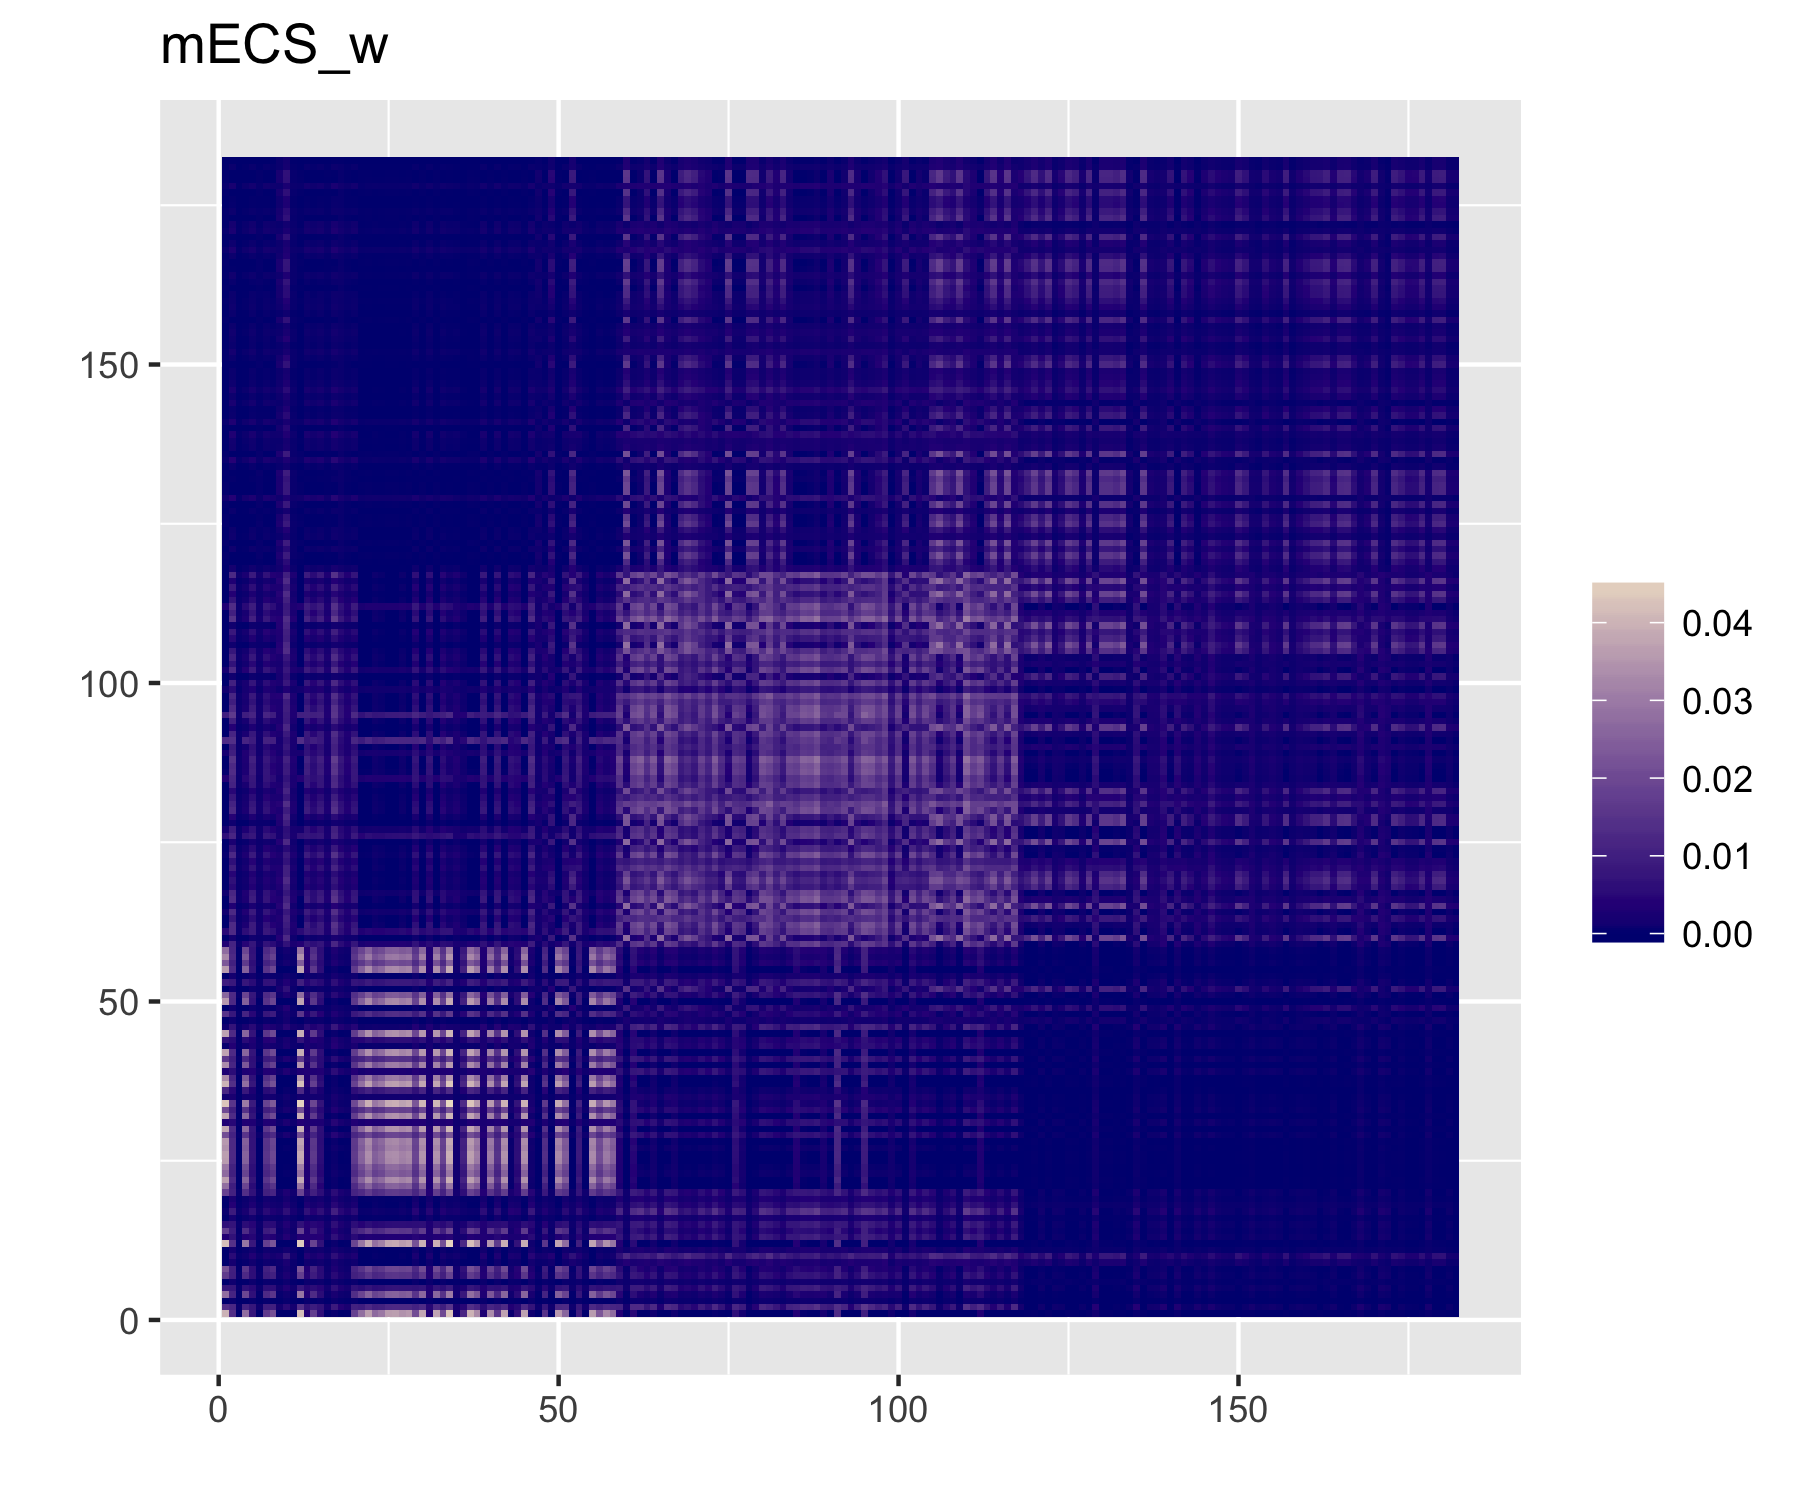
\includegraphics[width=0.33\linewidth]{mECS_w.png}
%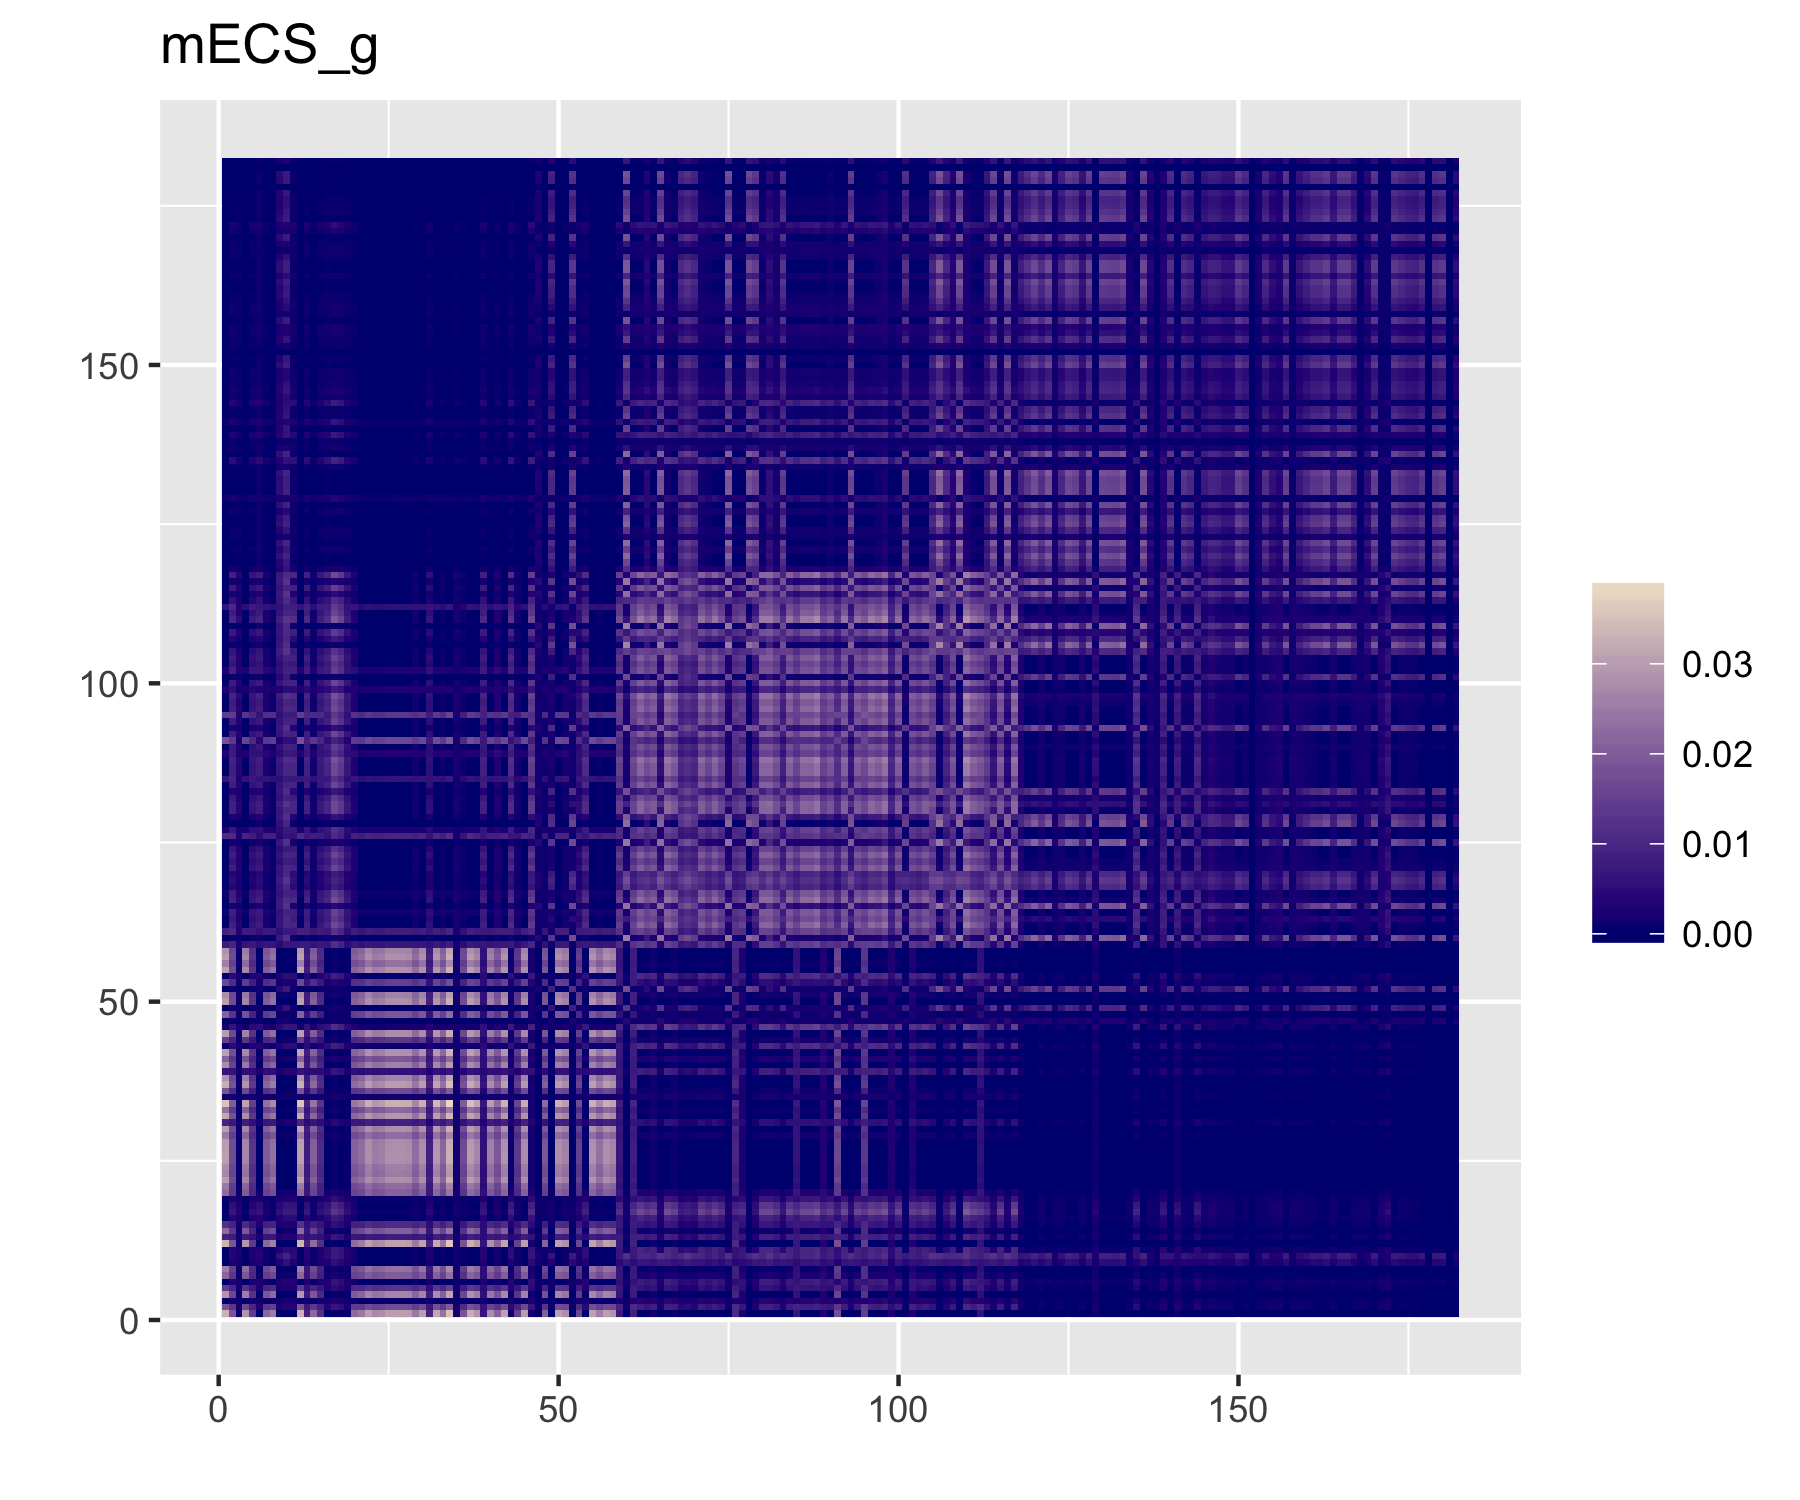
\includegraphics[width=0.33\linewidth]{mECS_g.png}
%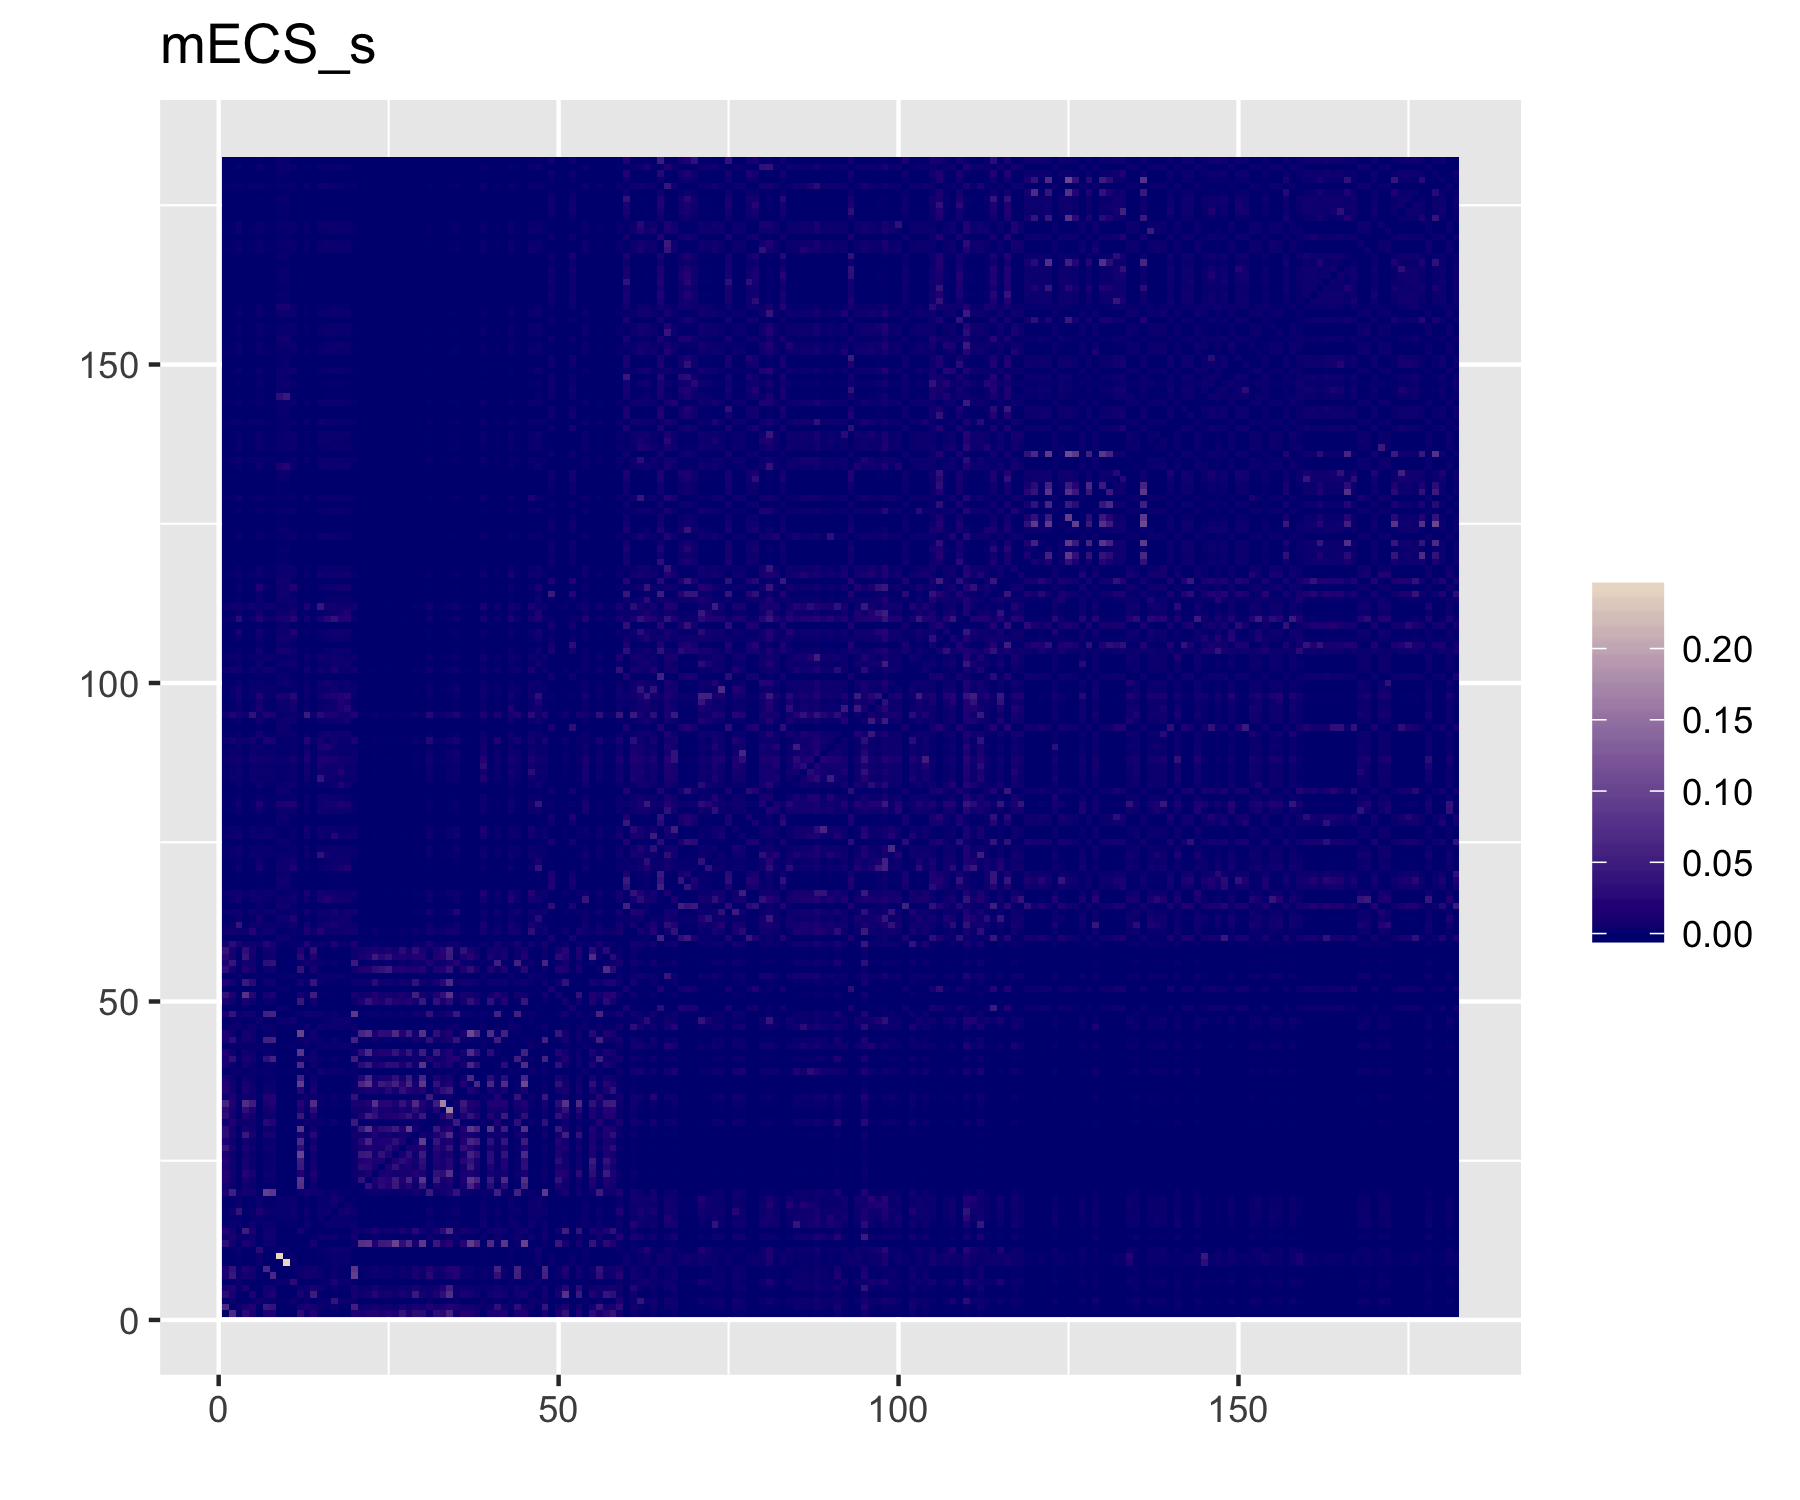
\includegraphics[width=0.33\linewidth]{mECS_s.png}
%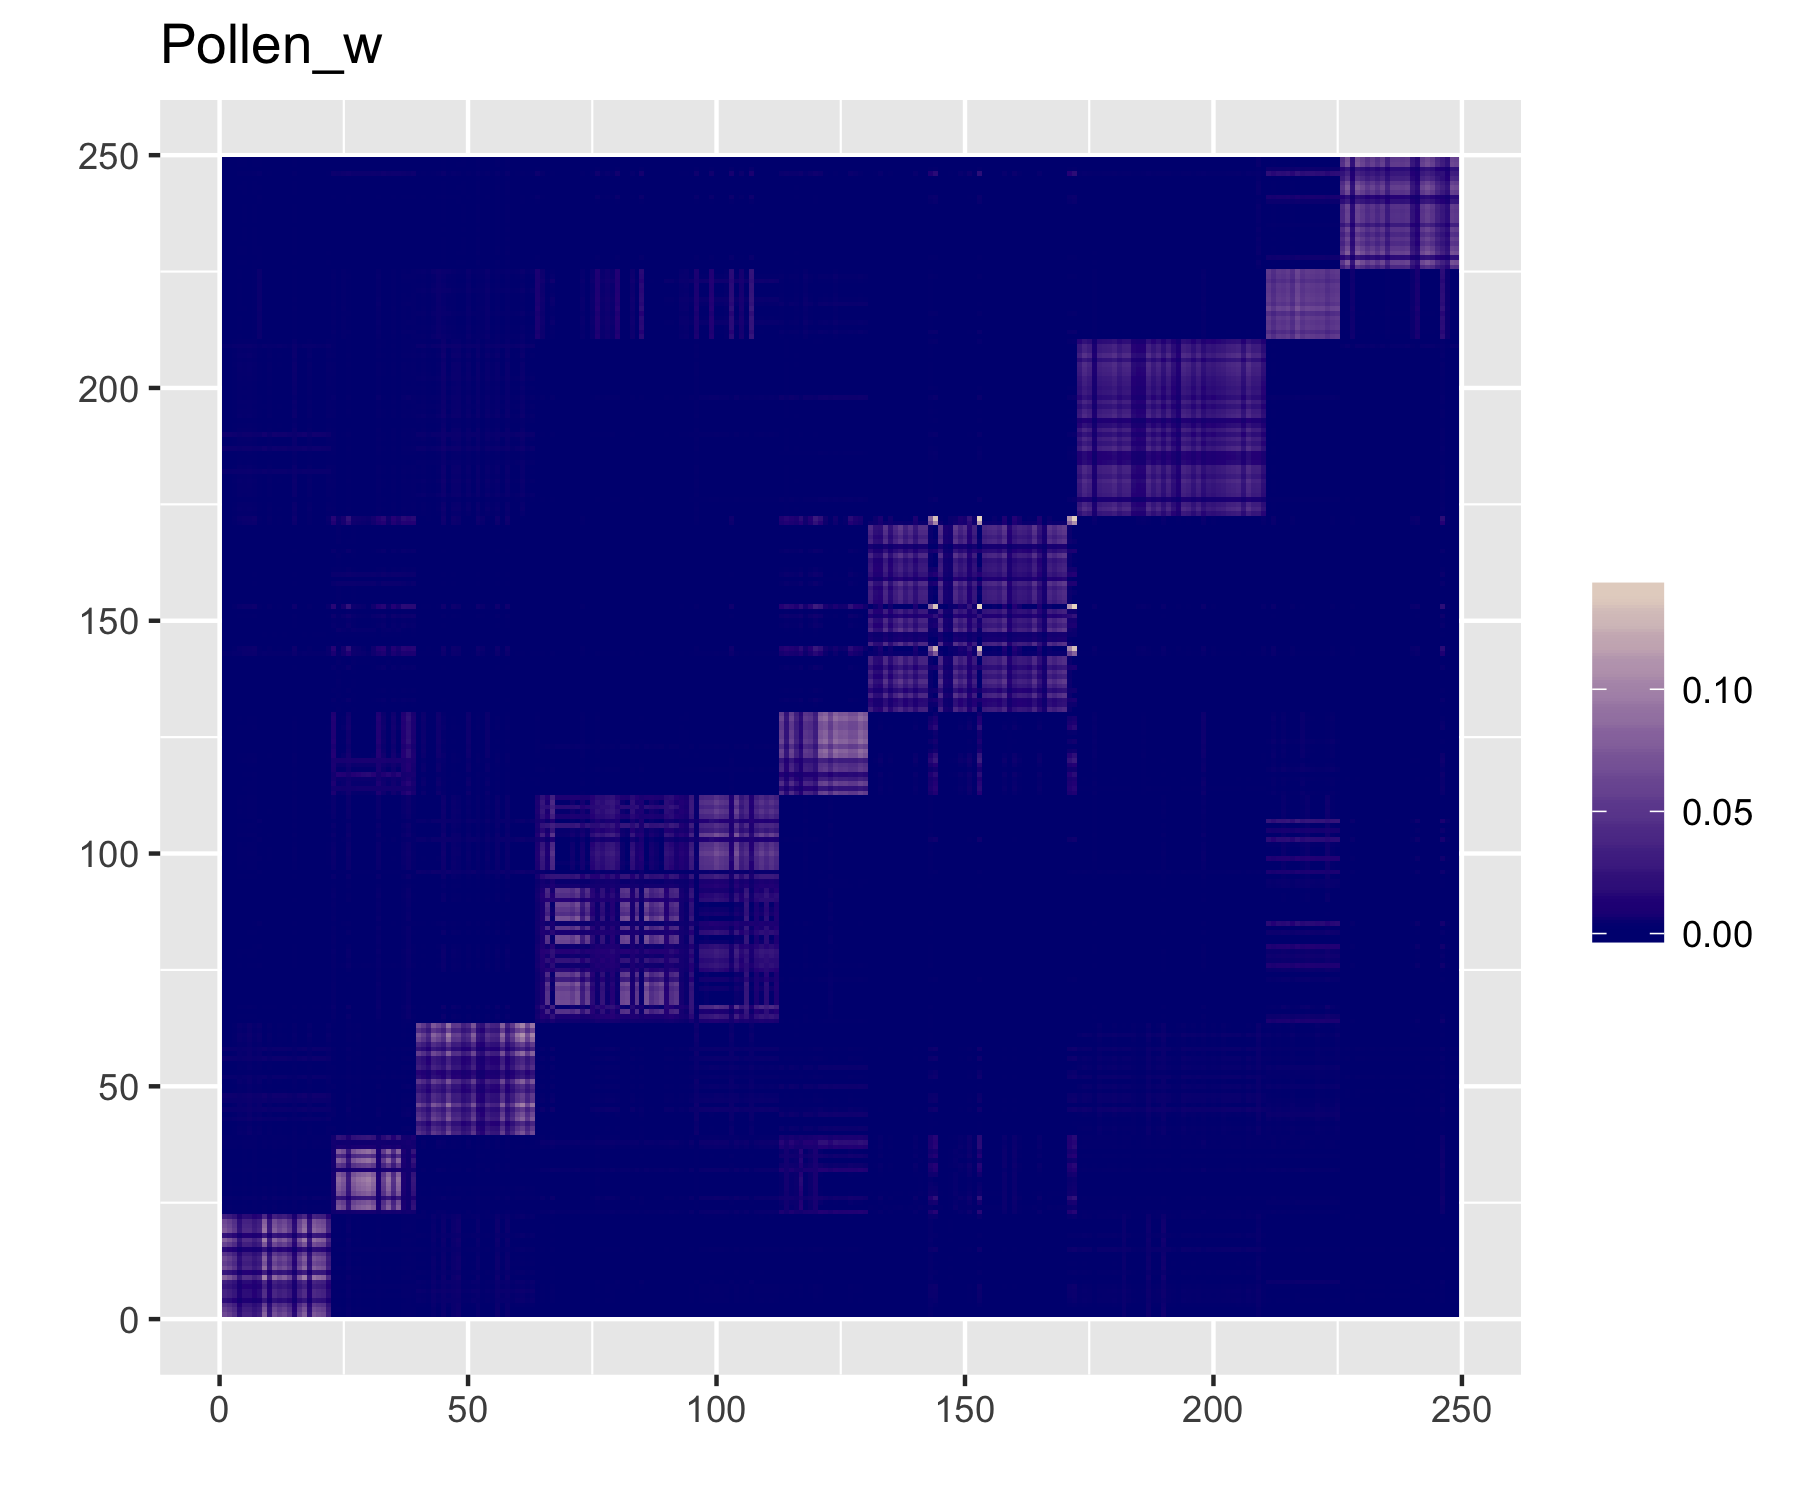
\includegraphics[width=0.33\linewidth]{Pollen_w.png}
%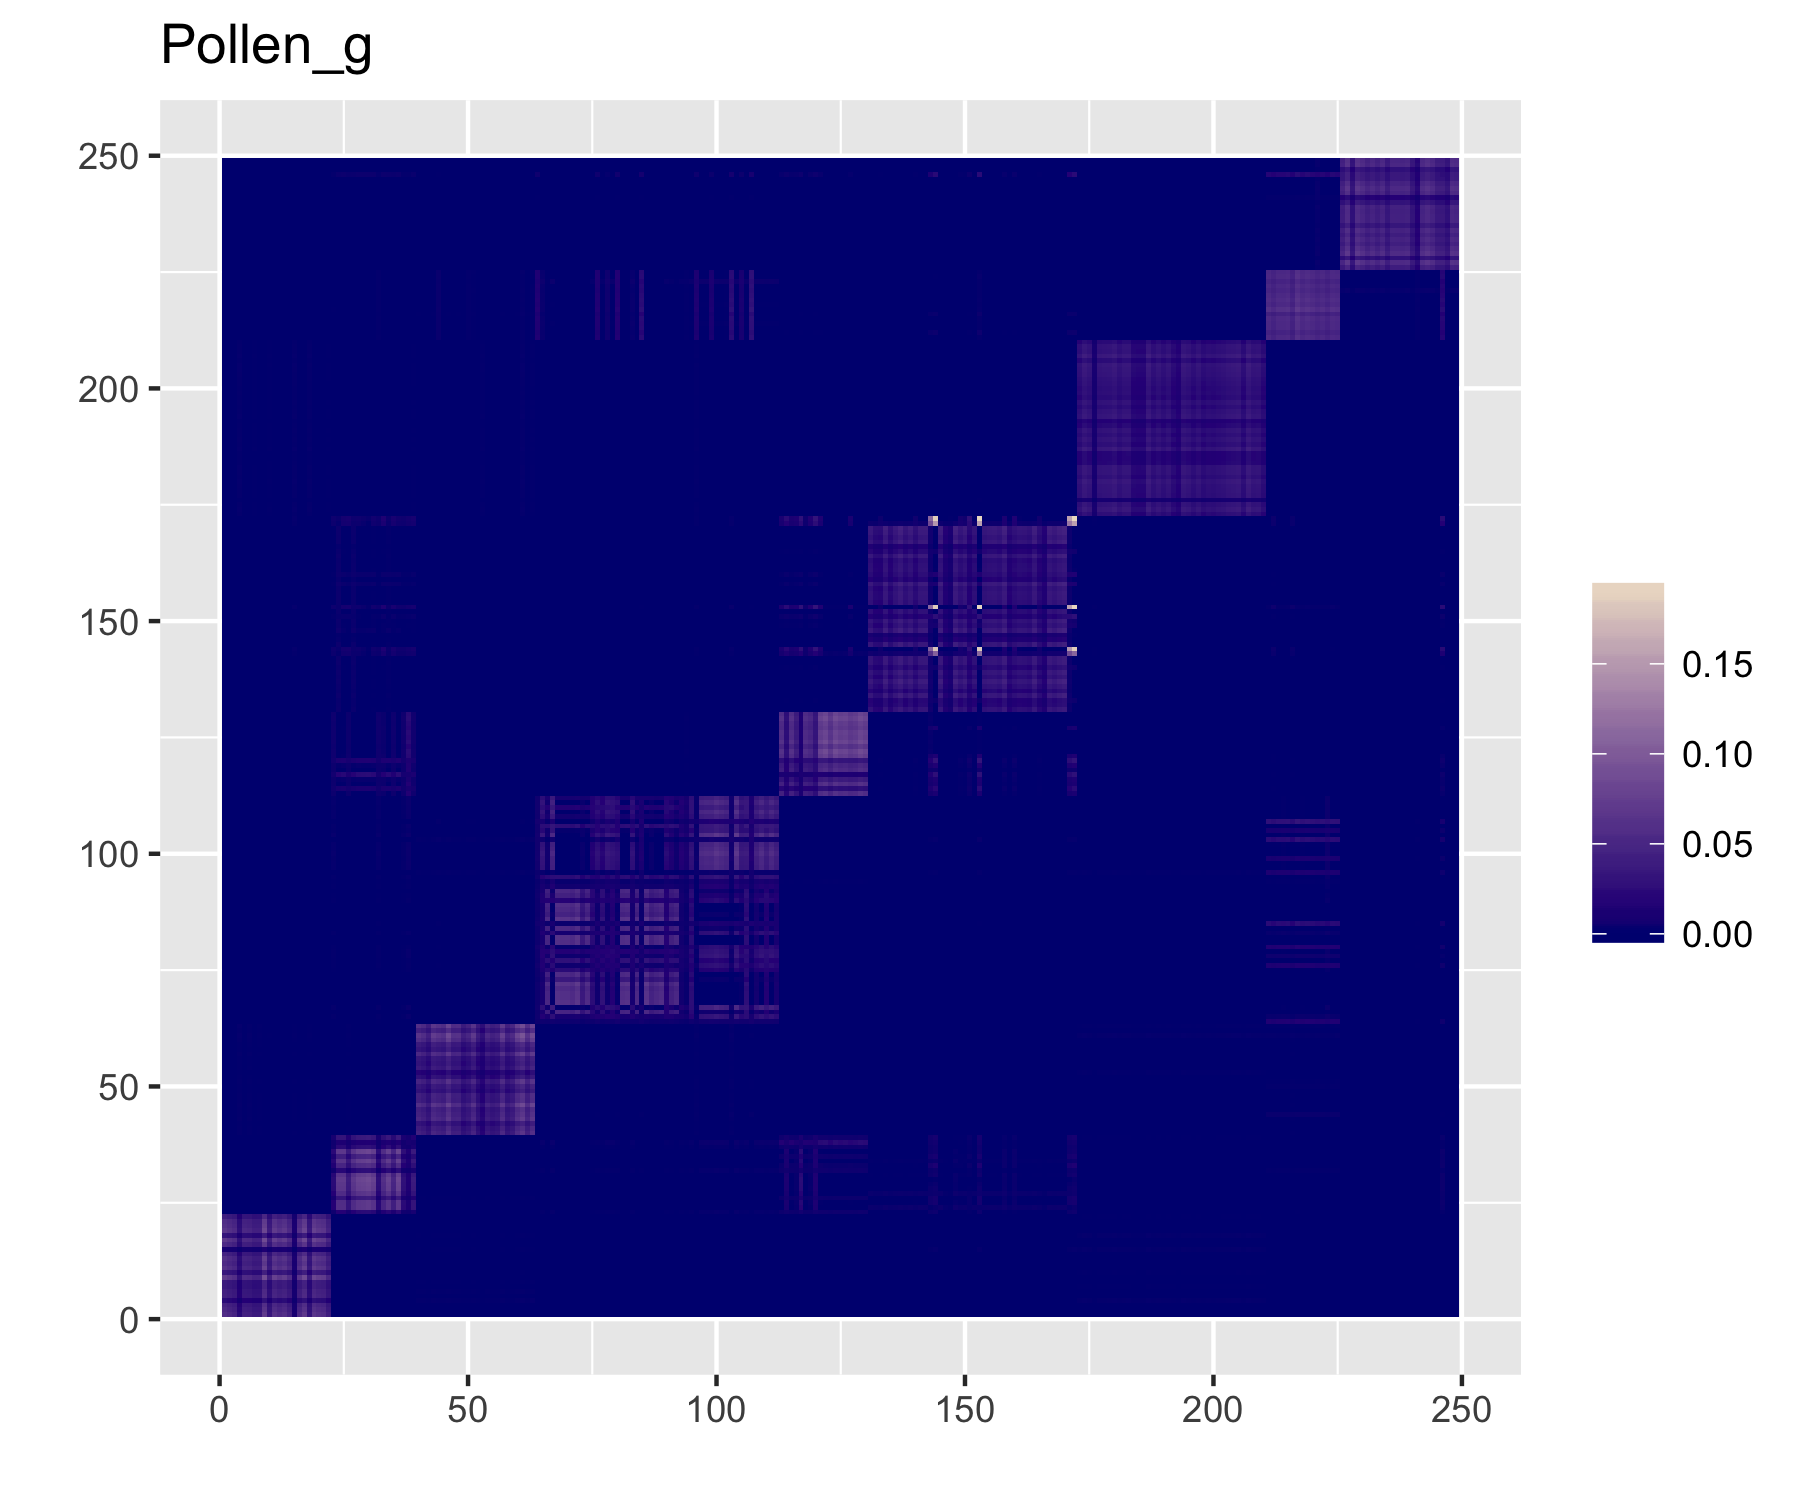
\includegraphics[width=0.33\linewidth]{Pollen_g.png}
%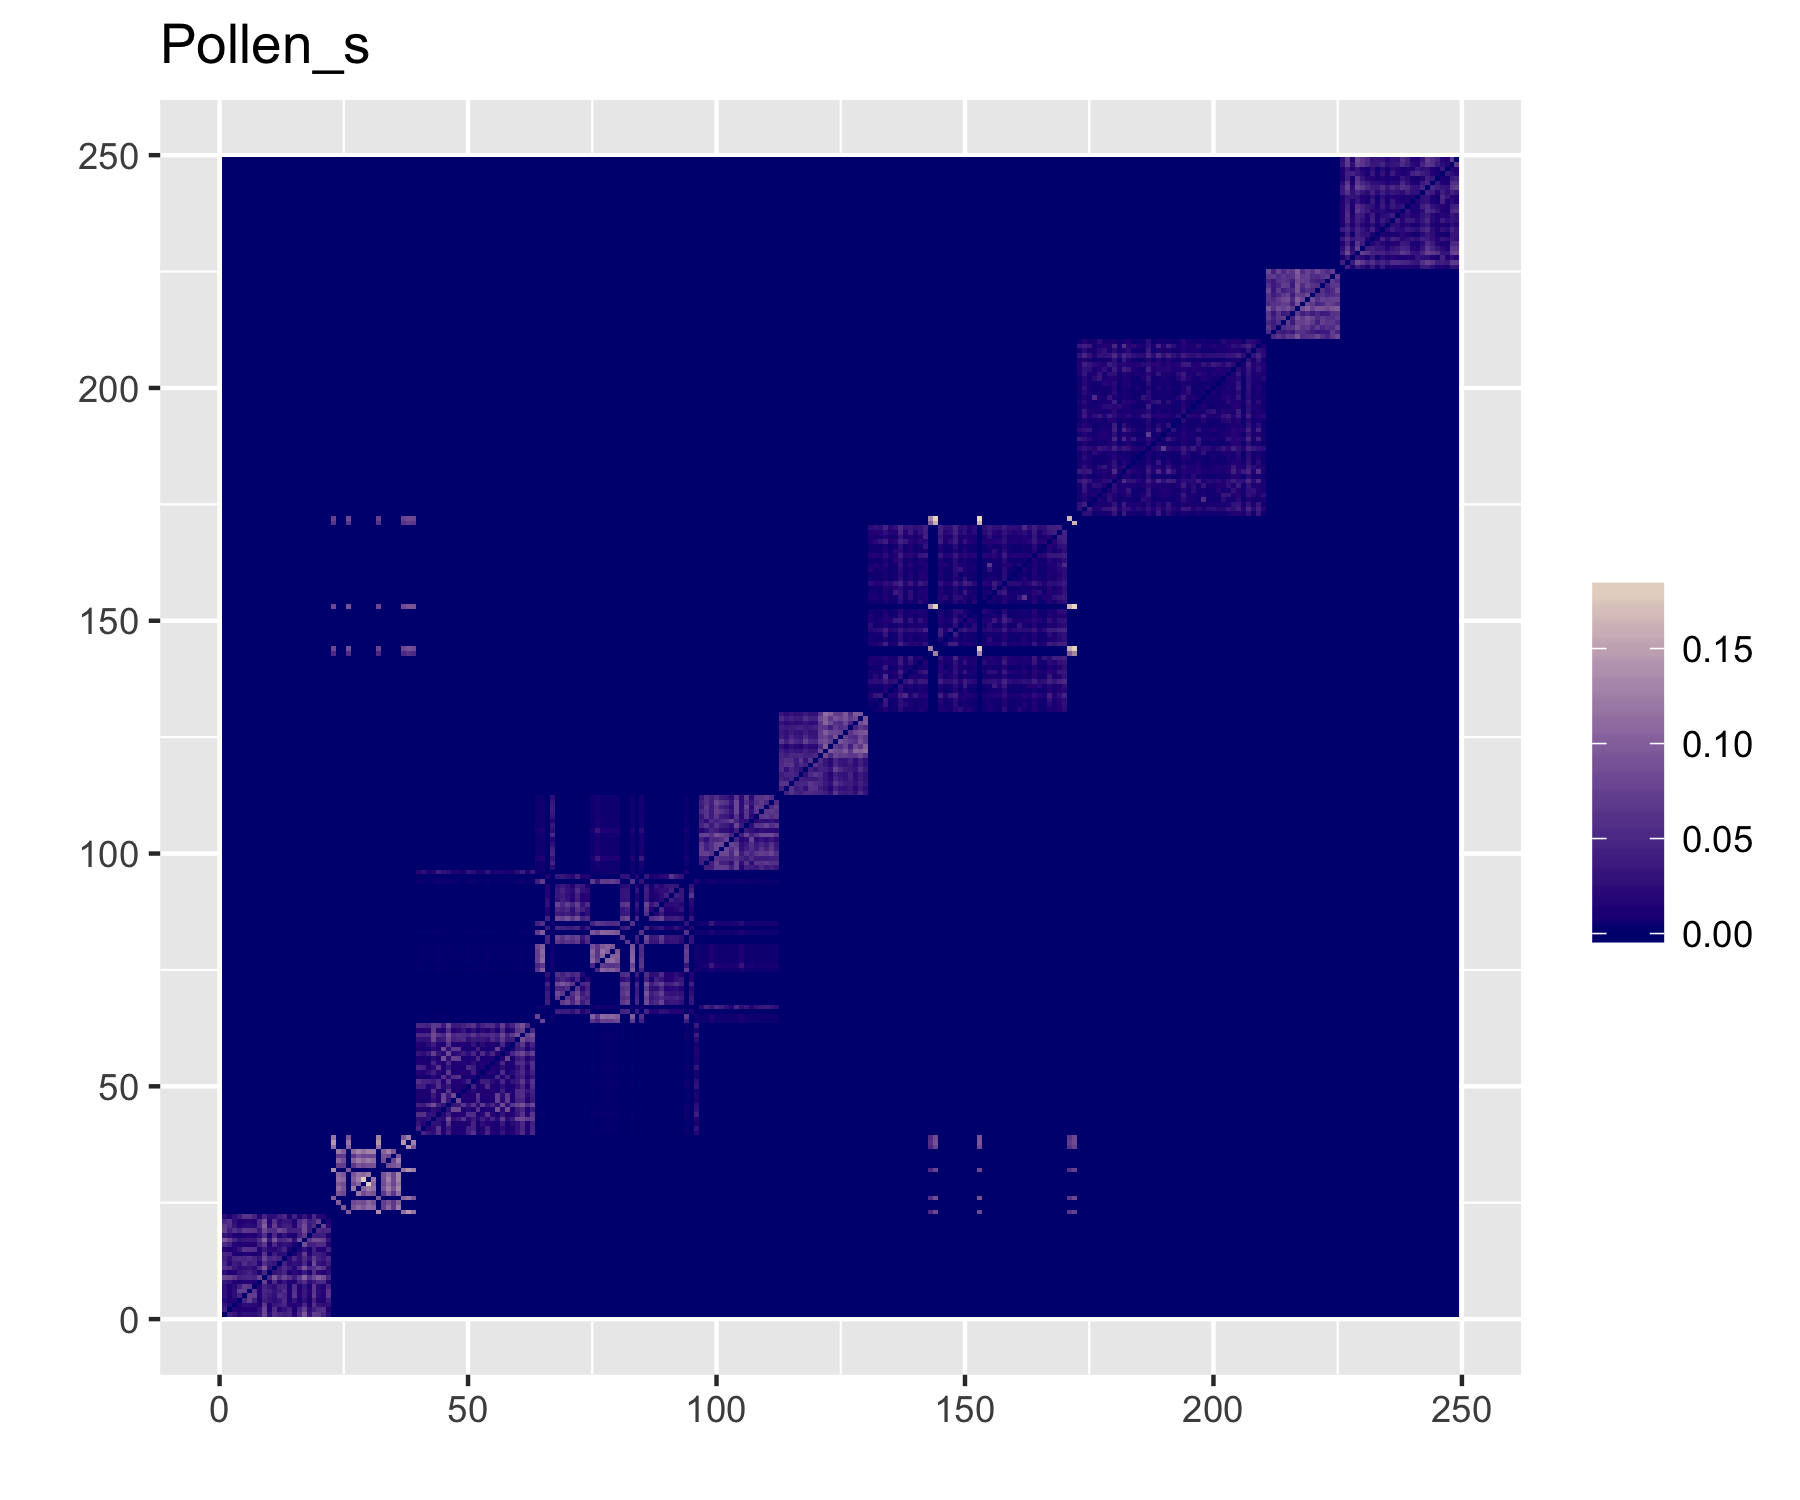
\includegraphics[width=0.33\linewidth]{Pollen_s.png}
%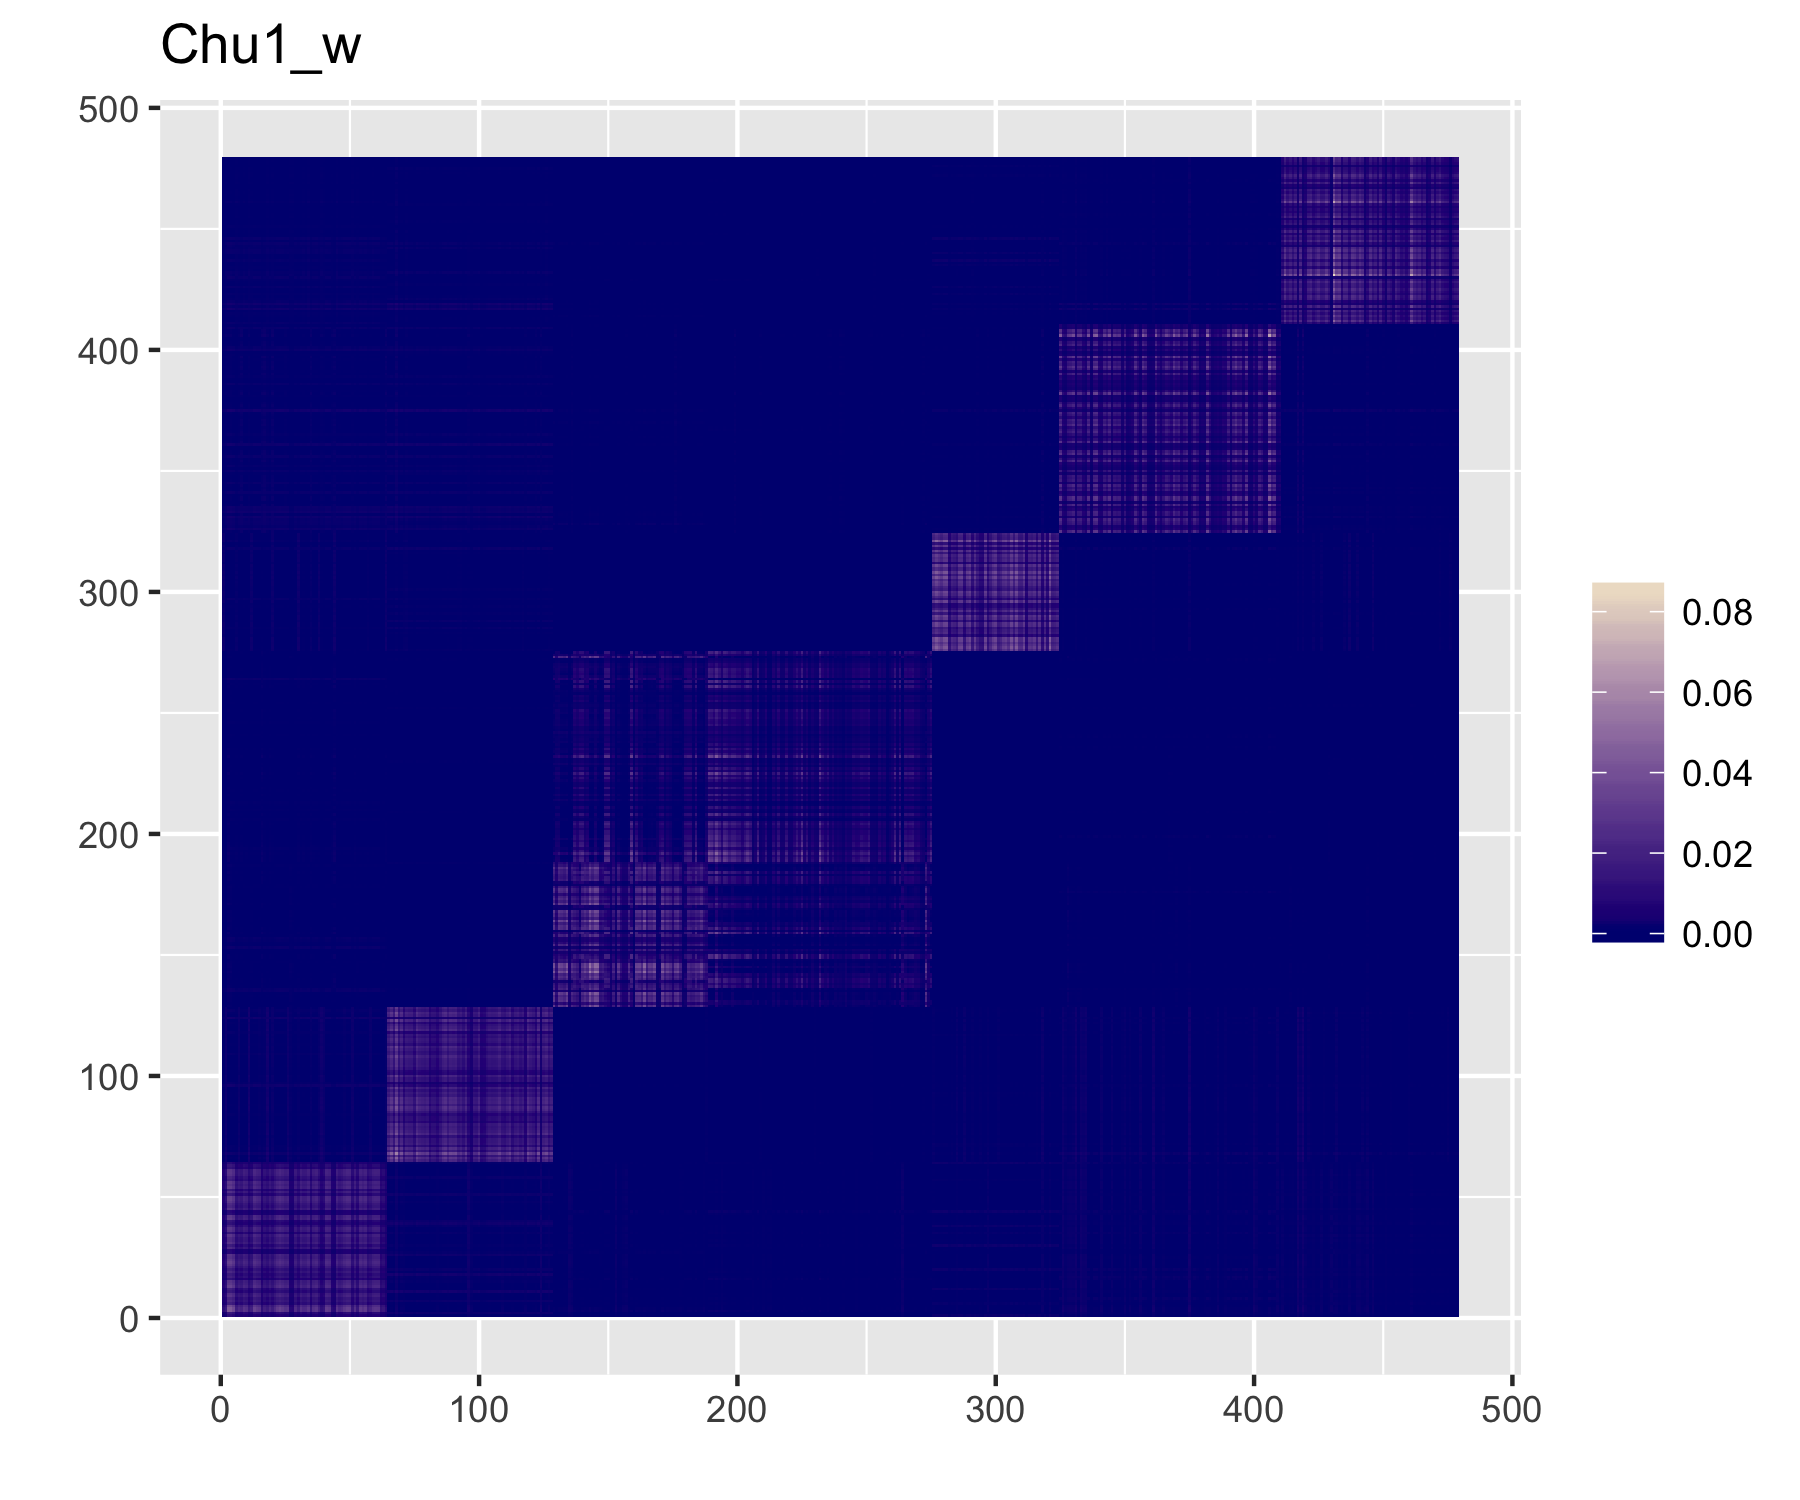
\includegraphics[width=0.33\linewidth]{Chu1_w.png}
%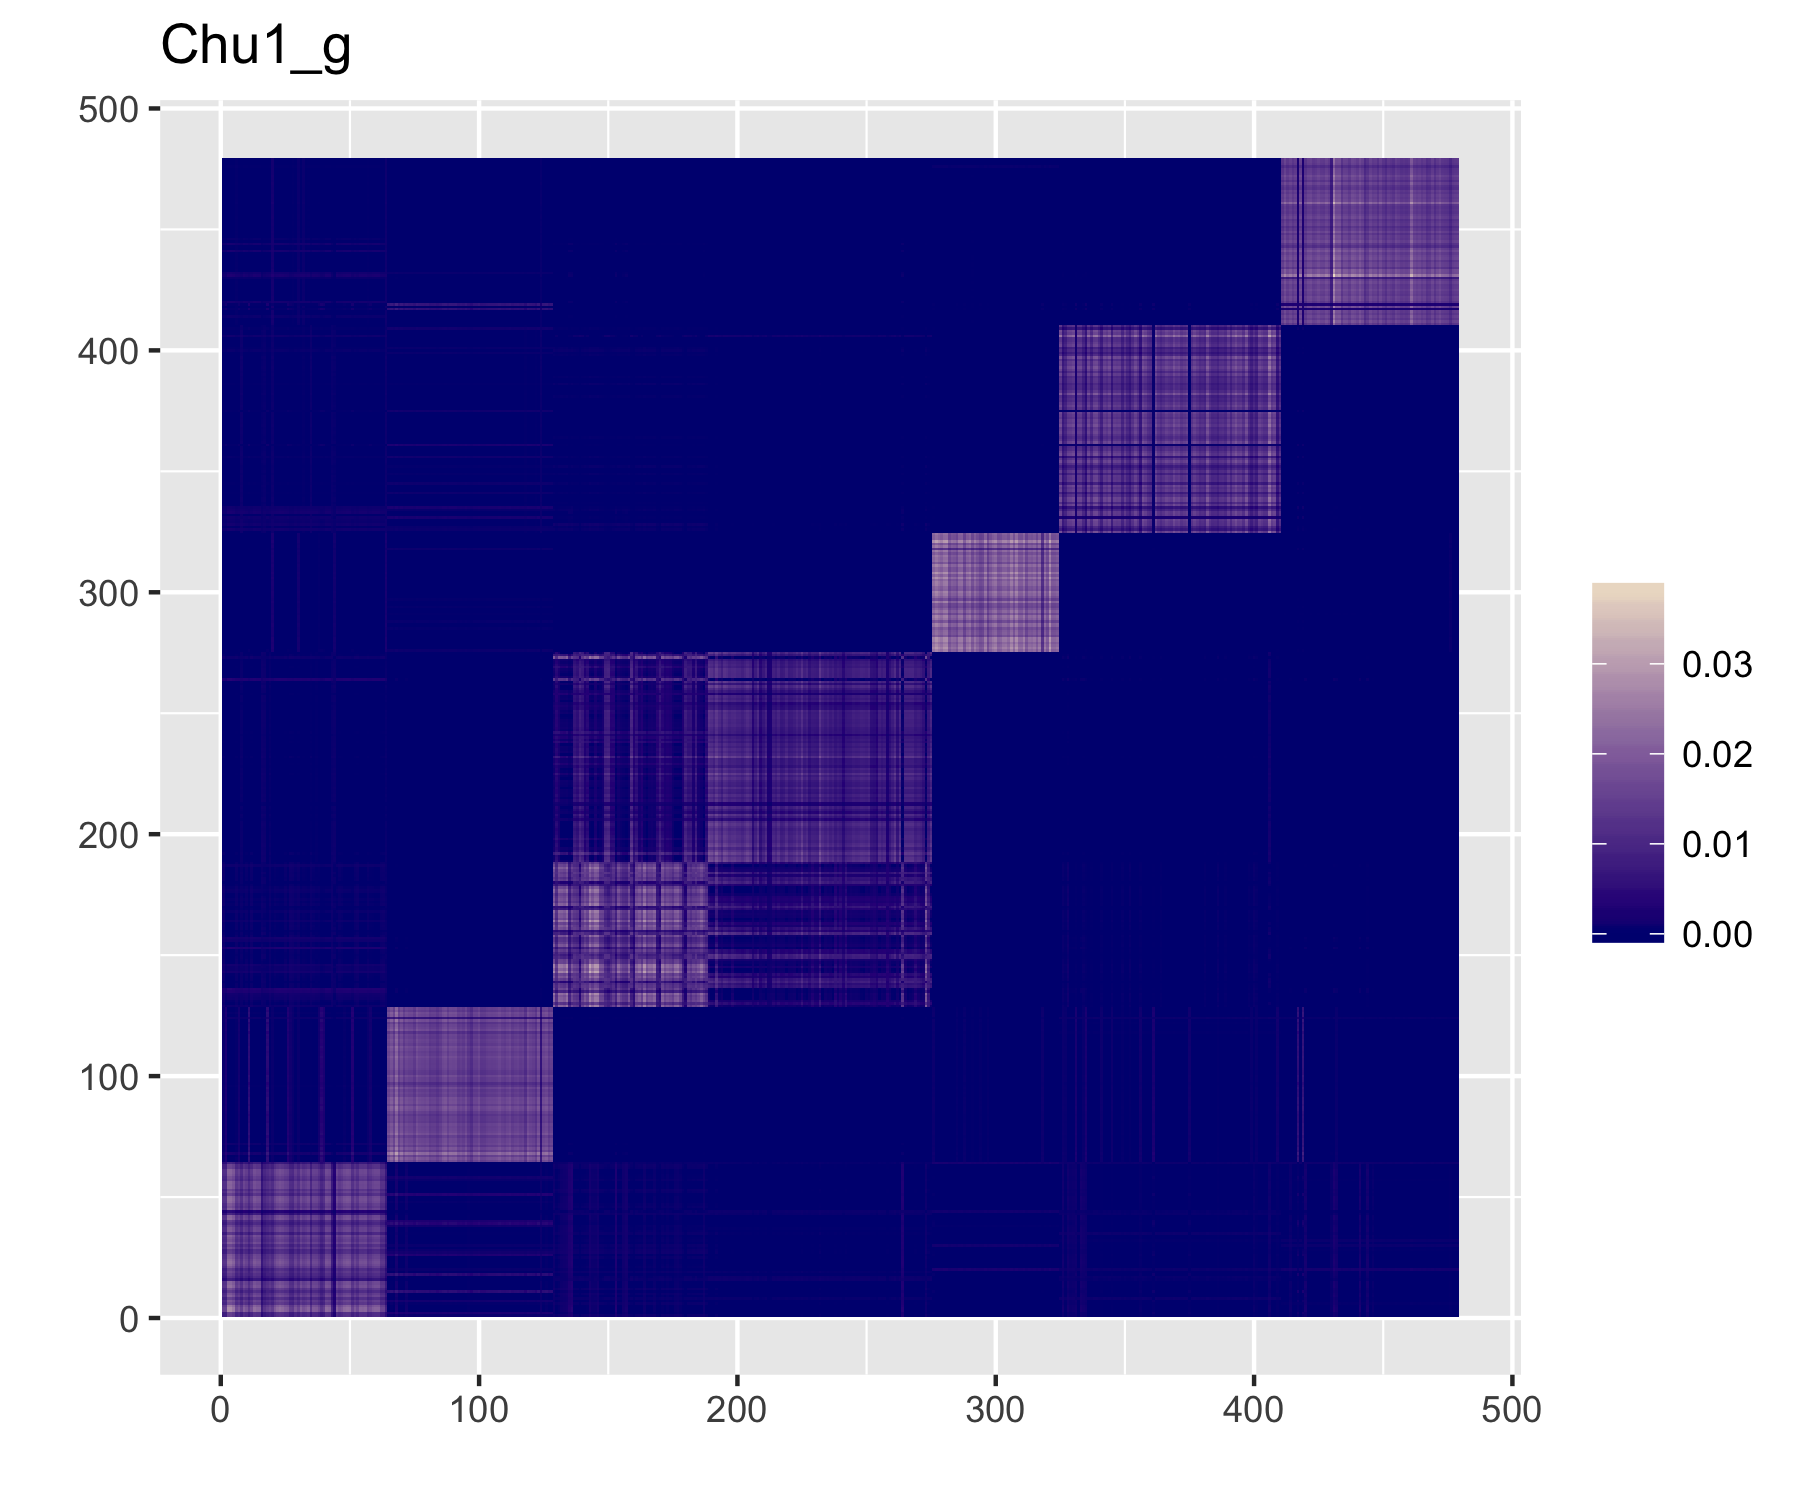
\includegraphics[width=0.33\linewidth]{Chu1_g.png}
%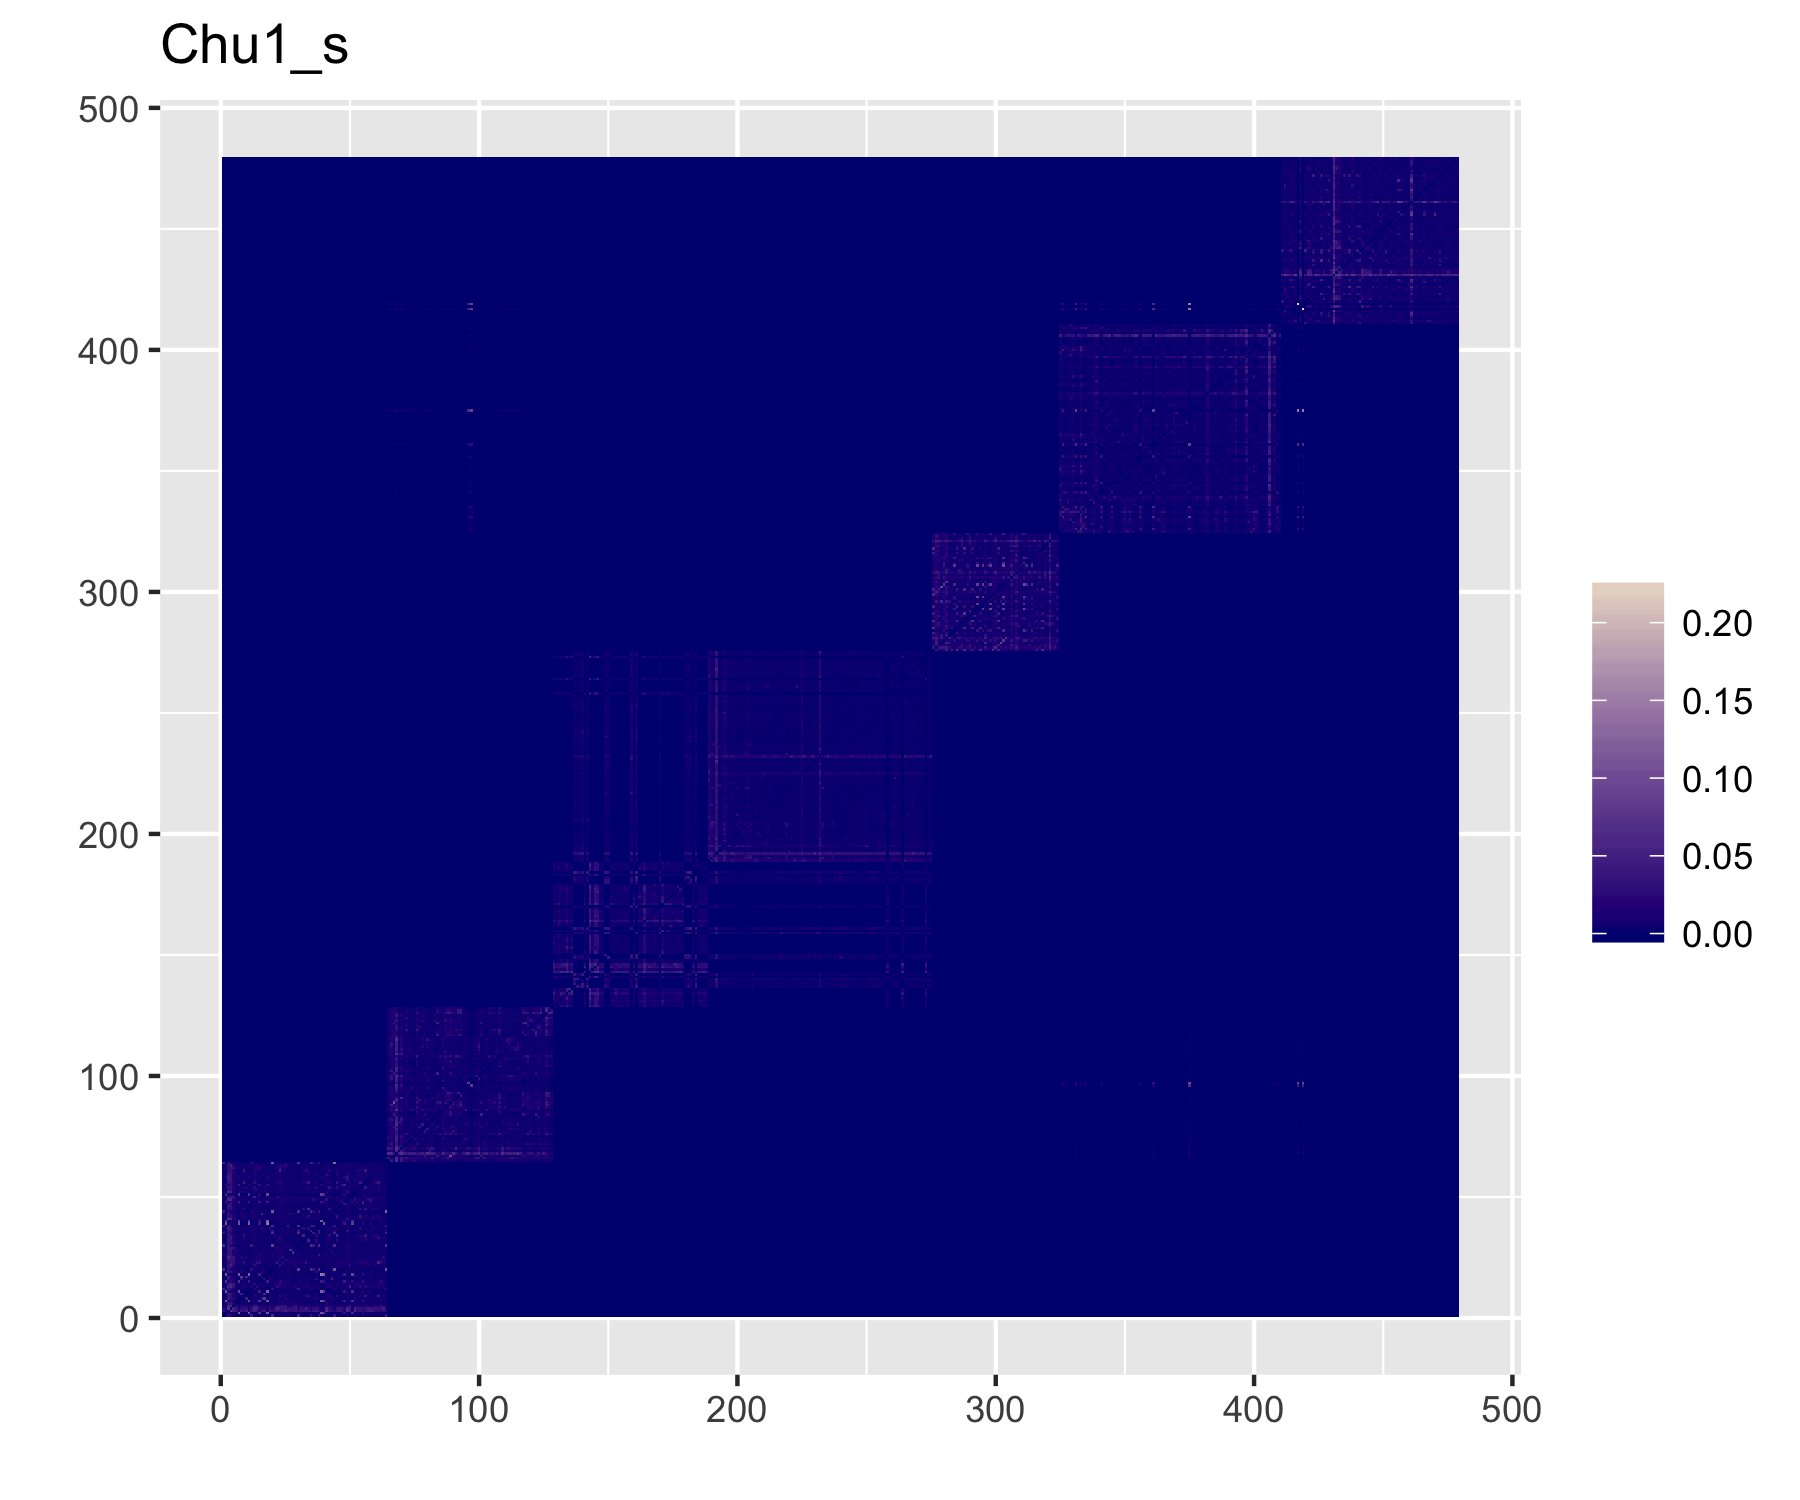
\includegraphics[width=0.33\linewidth]{Chu1_s.png}
%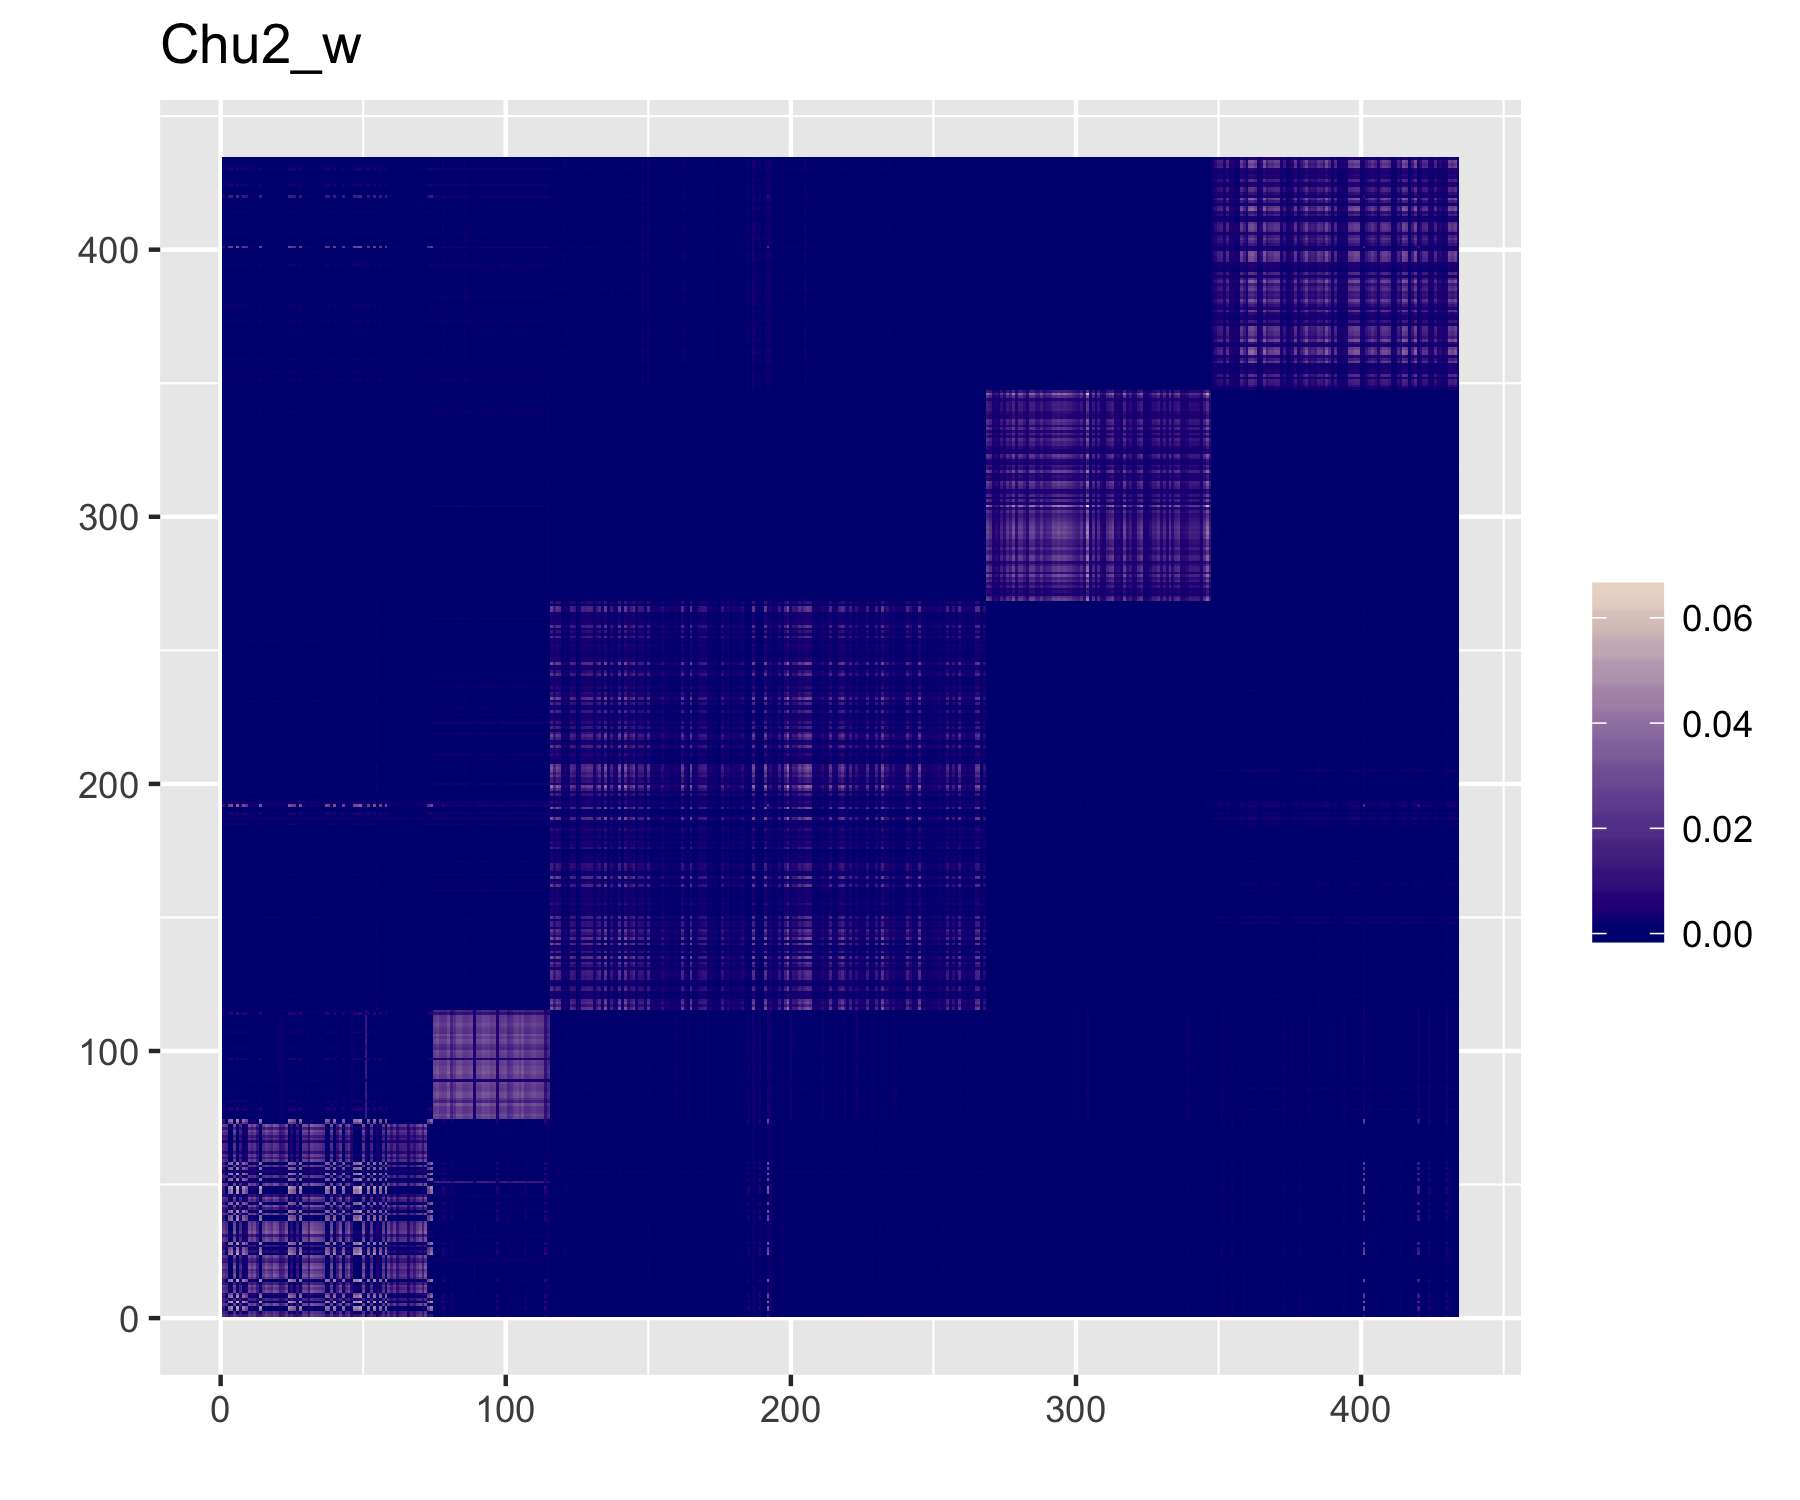
\includegraphics[width=0.33\linewidth]{Chu2_w.png}
%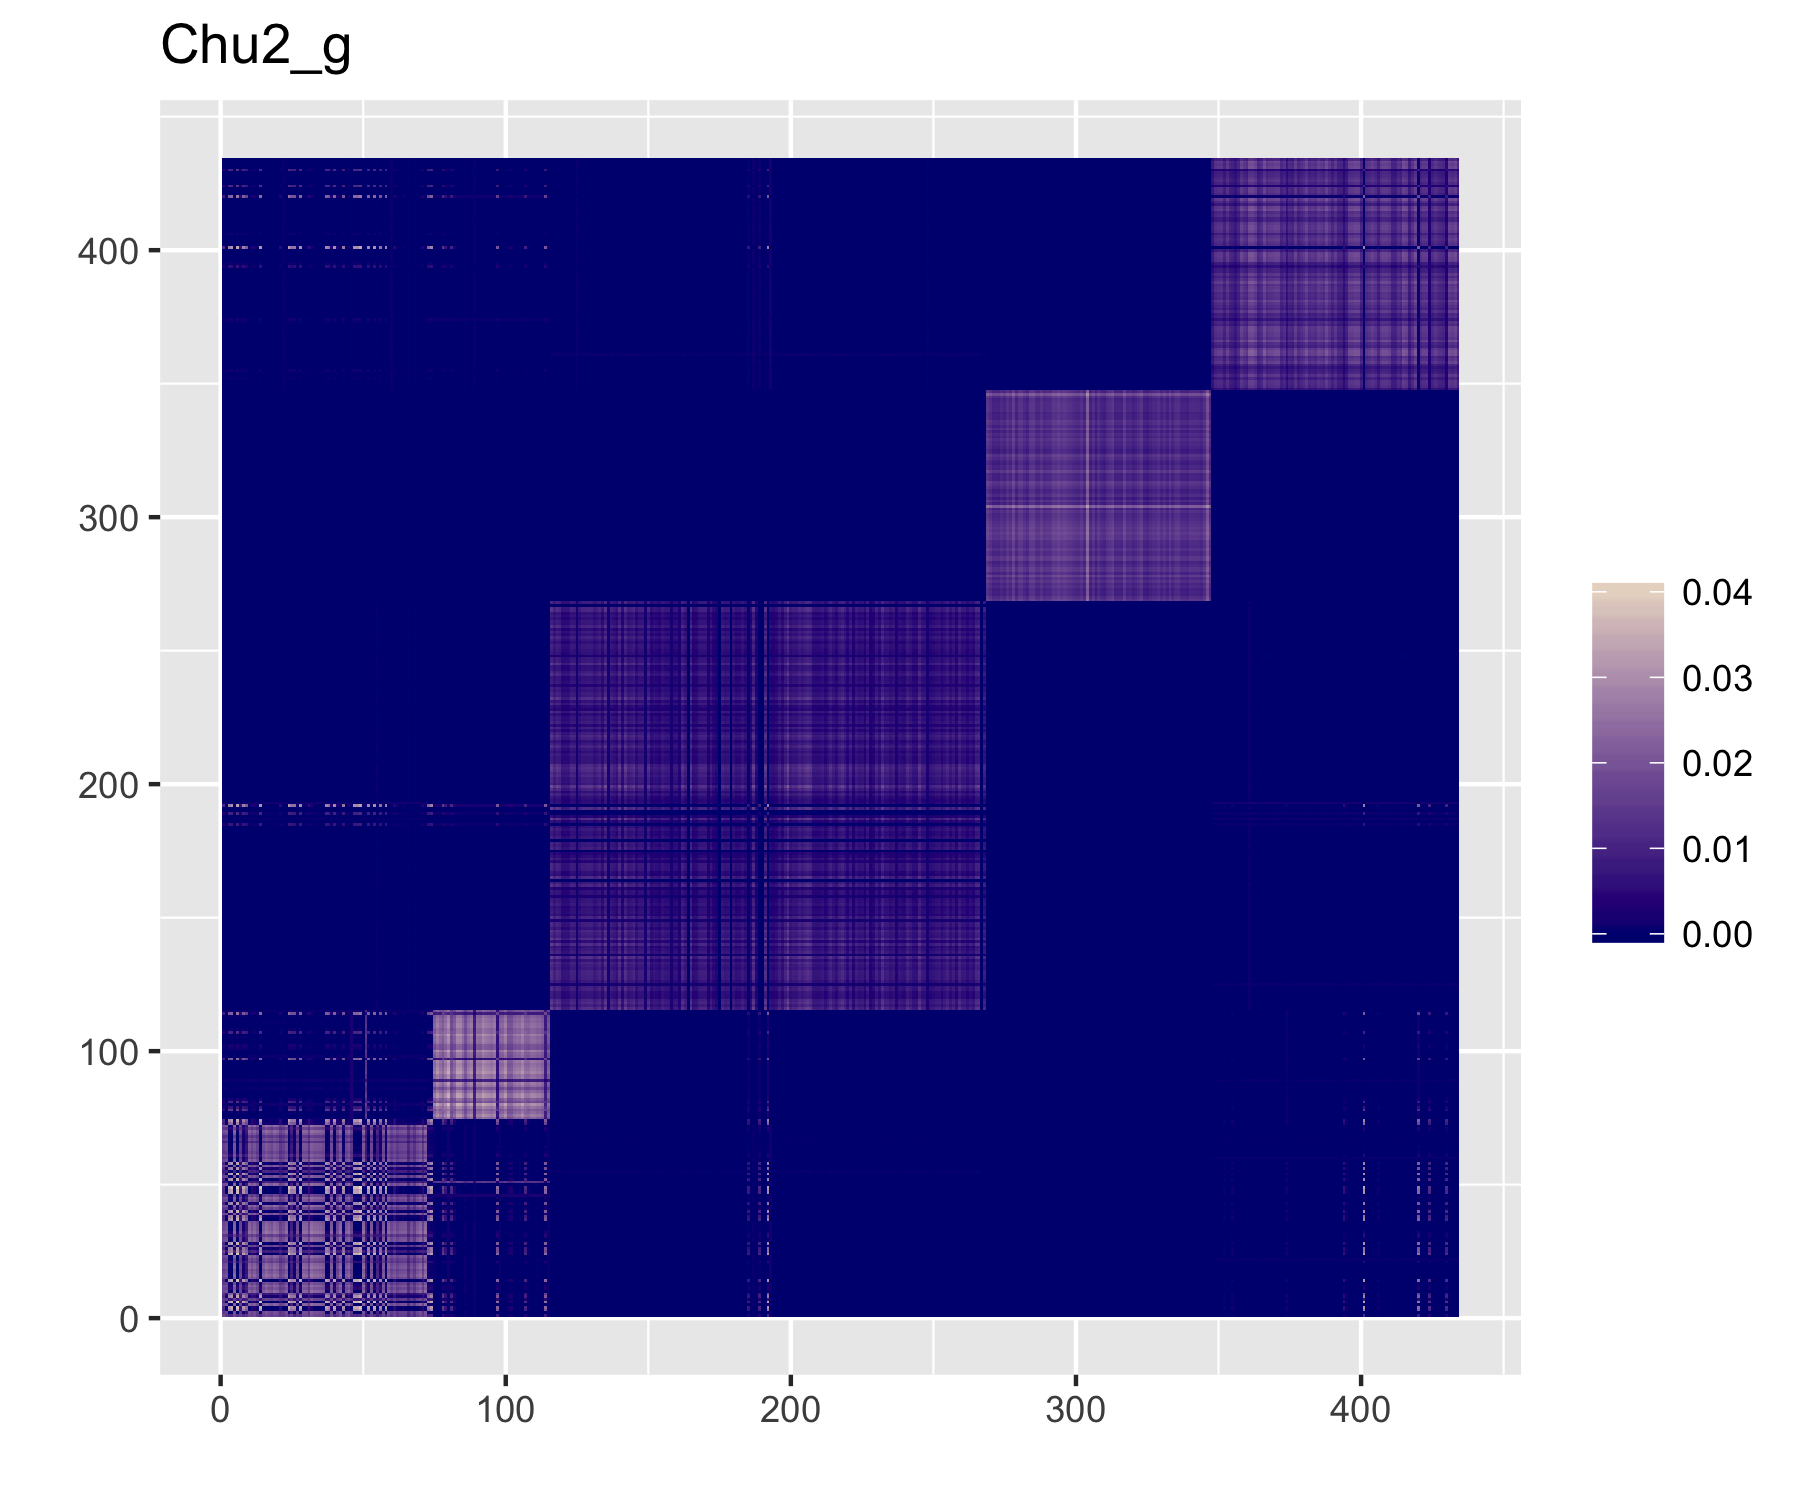
\includegraphics[width=0.33\linewidth]{Chu2_g.png}
%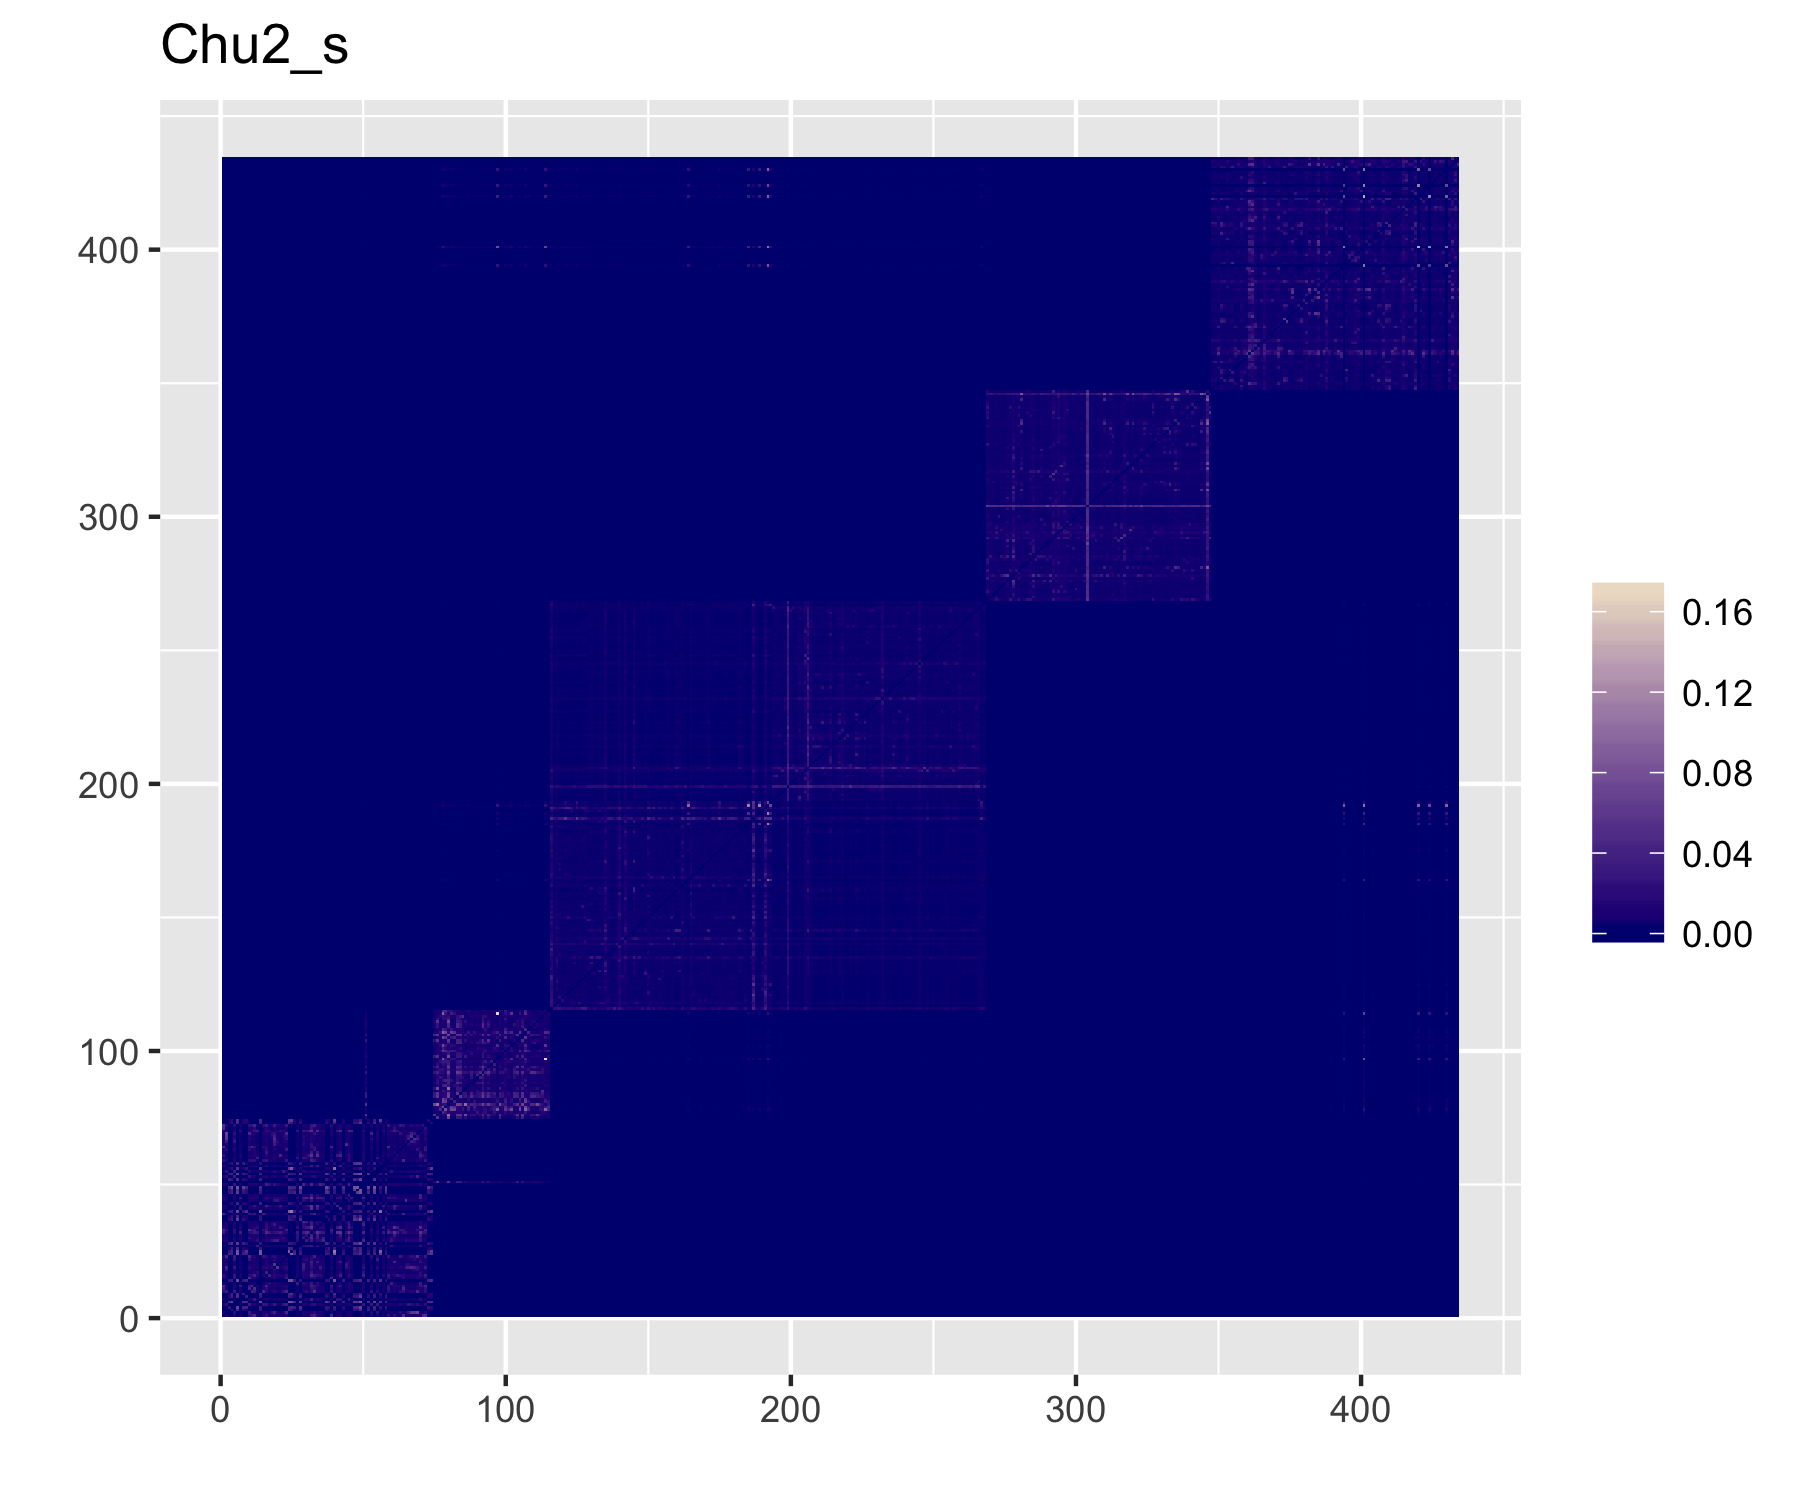
\includegraphics[width=0.33\linewidth]{Chu2_s.png}
%\end{figure}




%\begin{figure}[h]
%\centering
%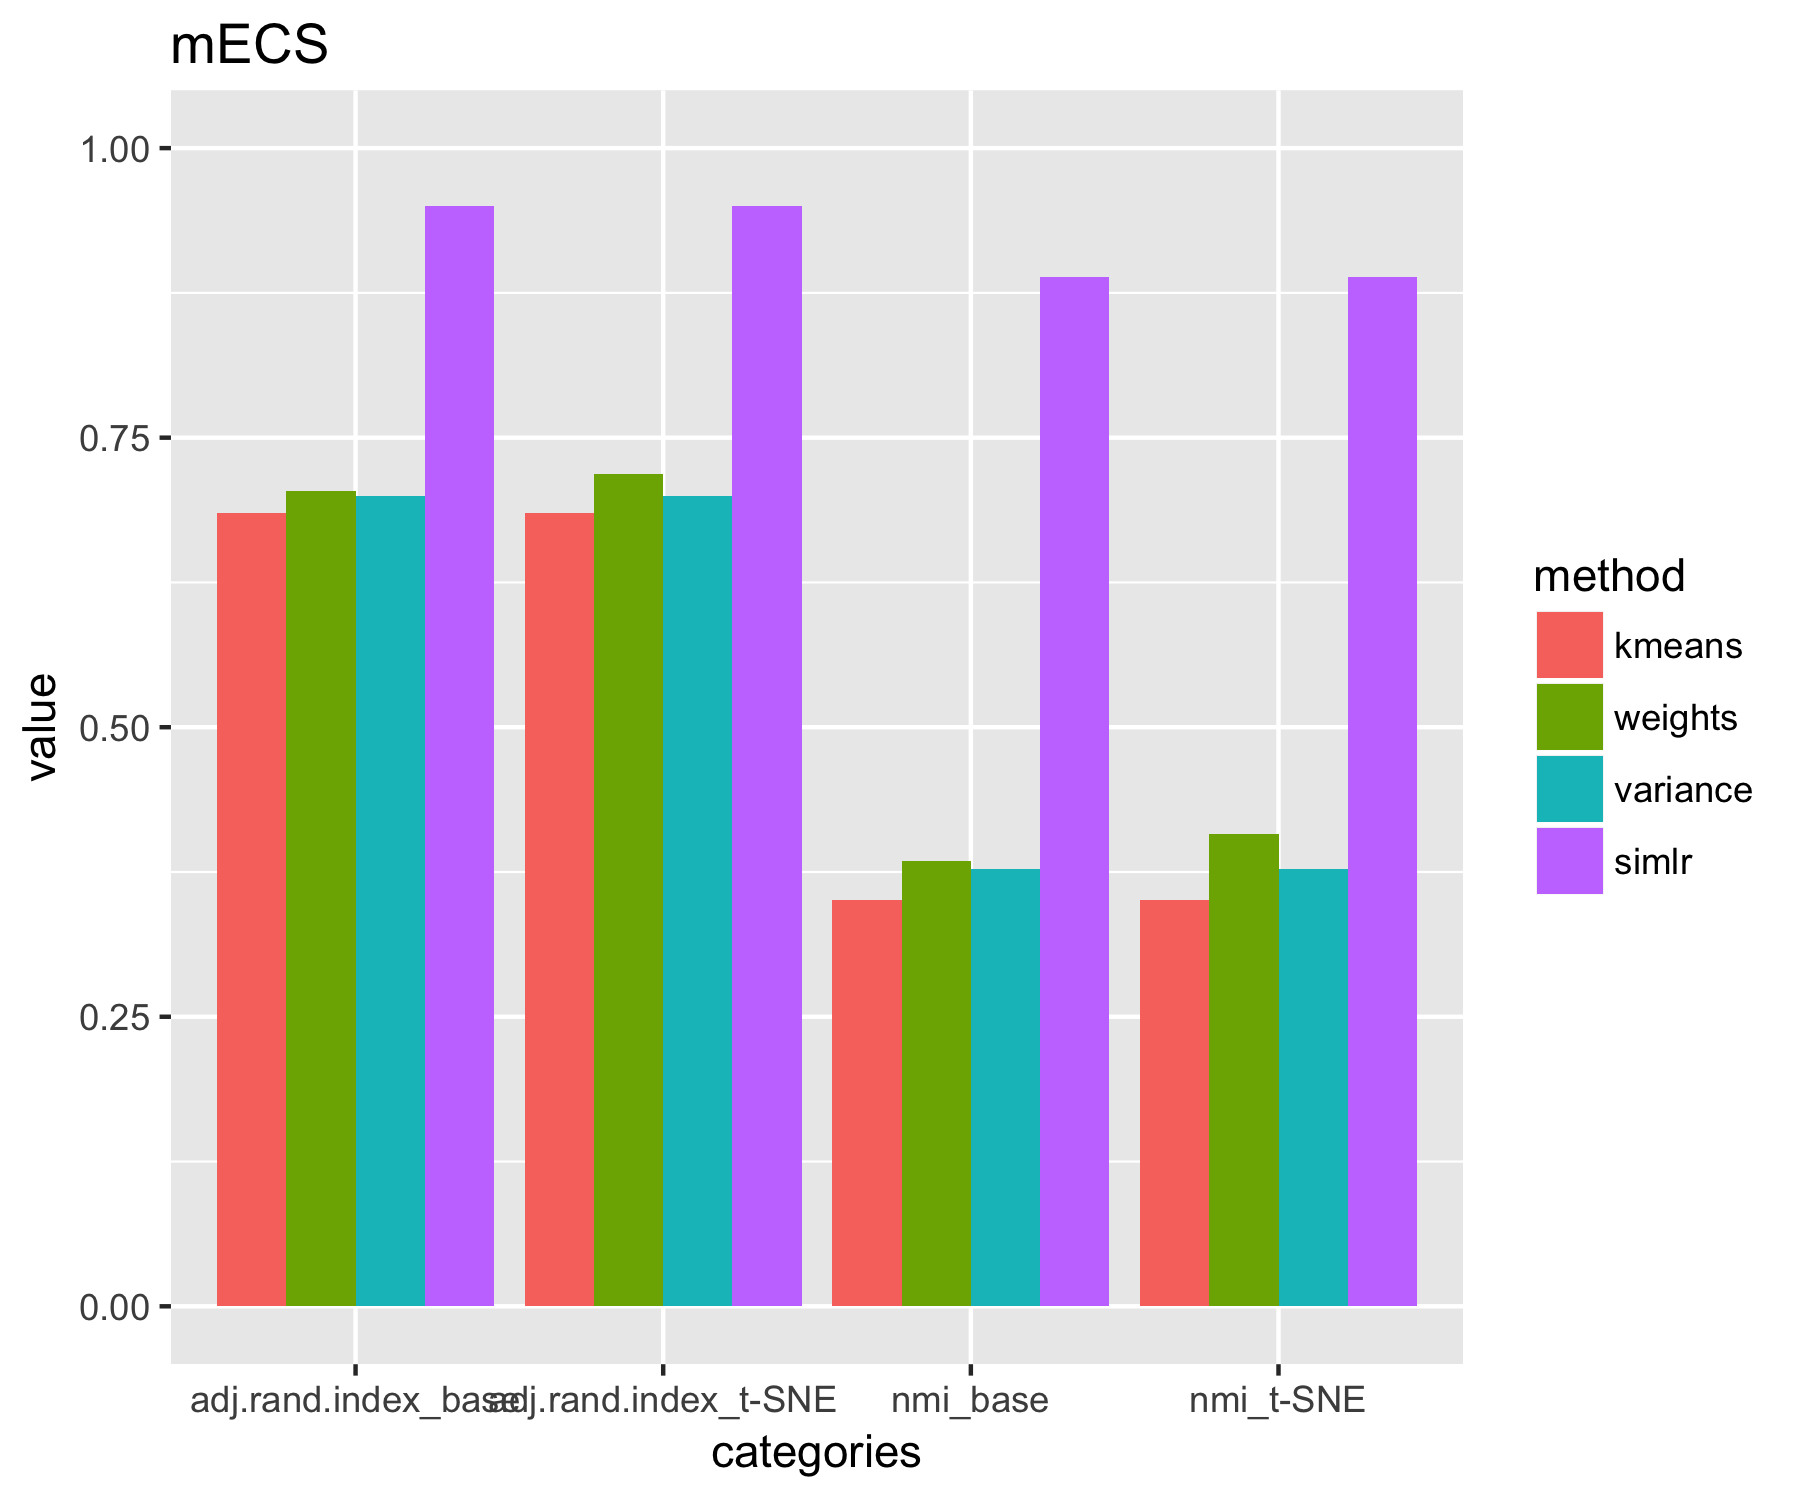
\includegraphics[width=0.45\linewidth]{mECS_performance.png}
%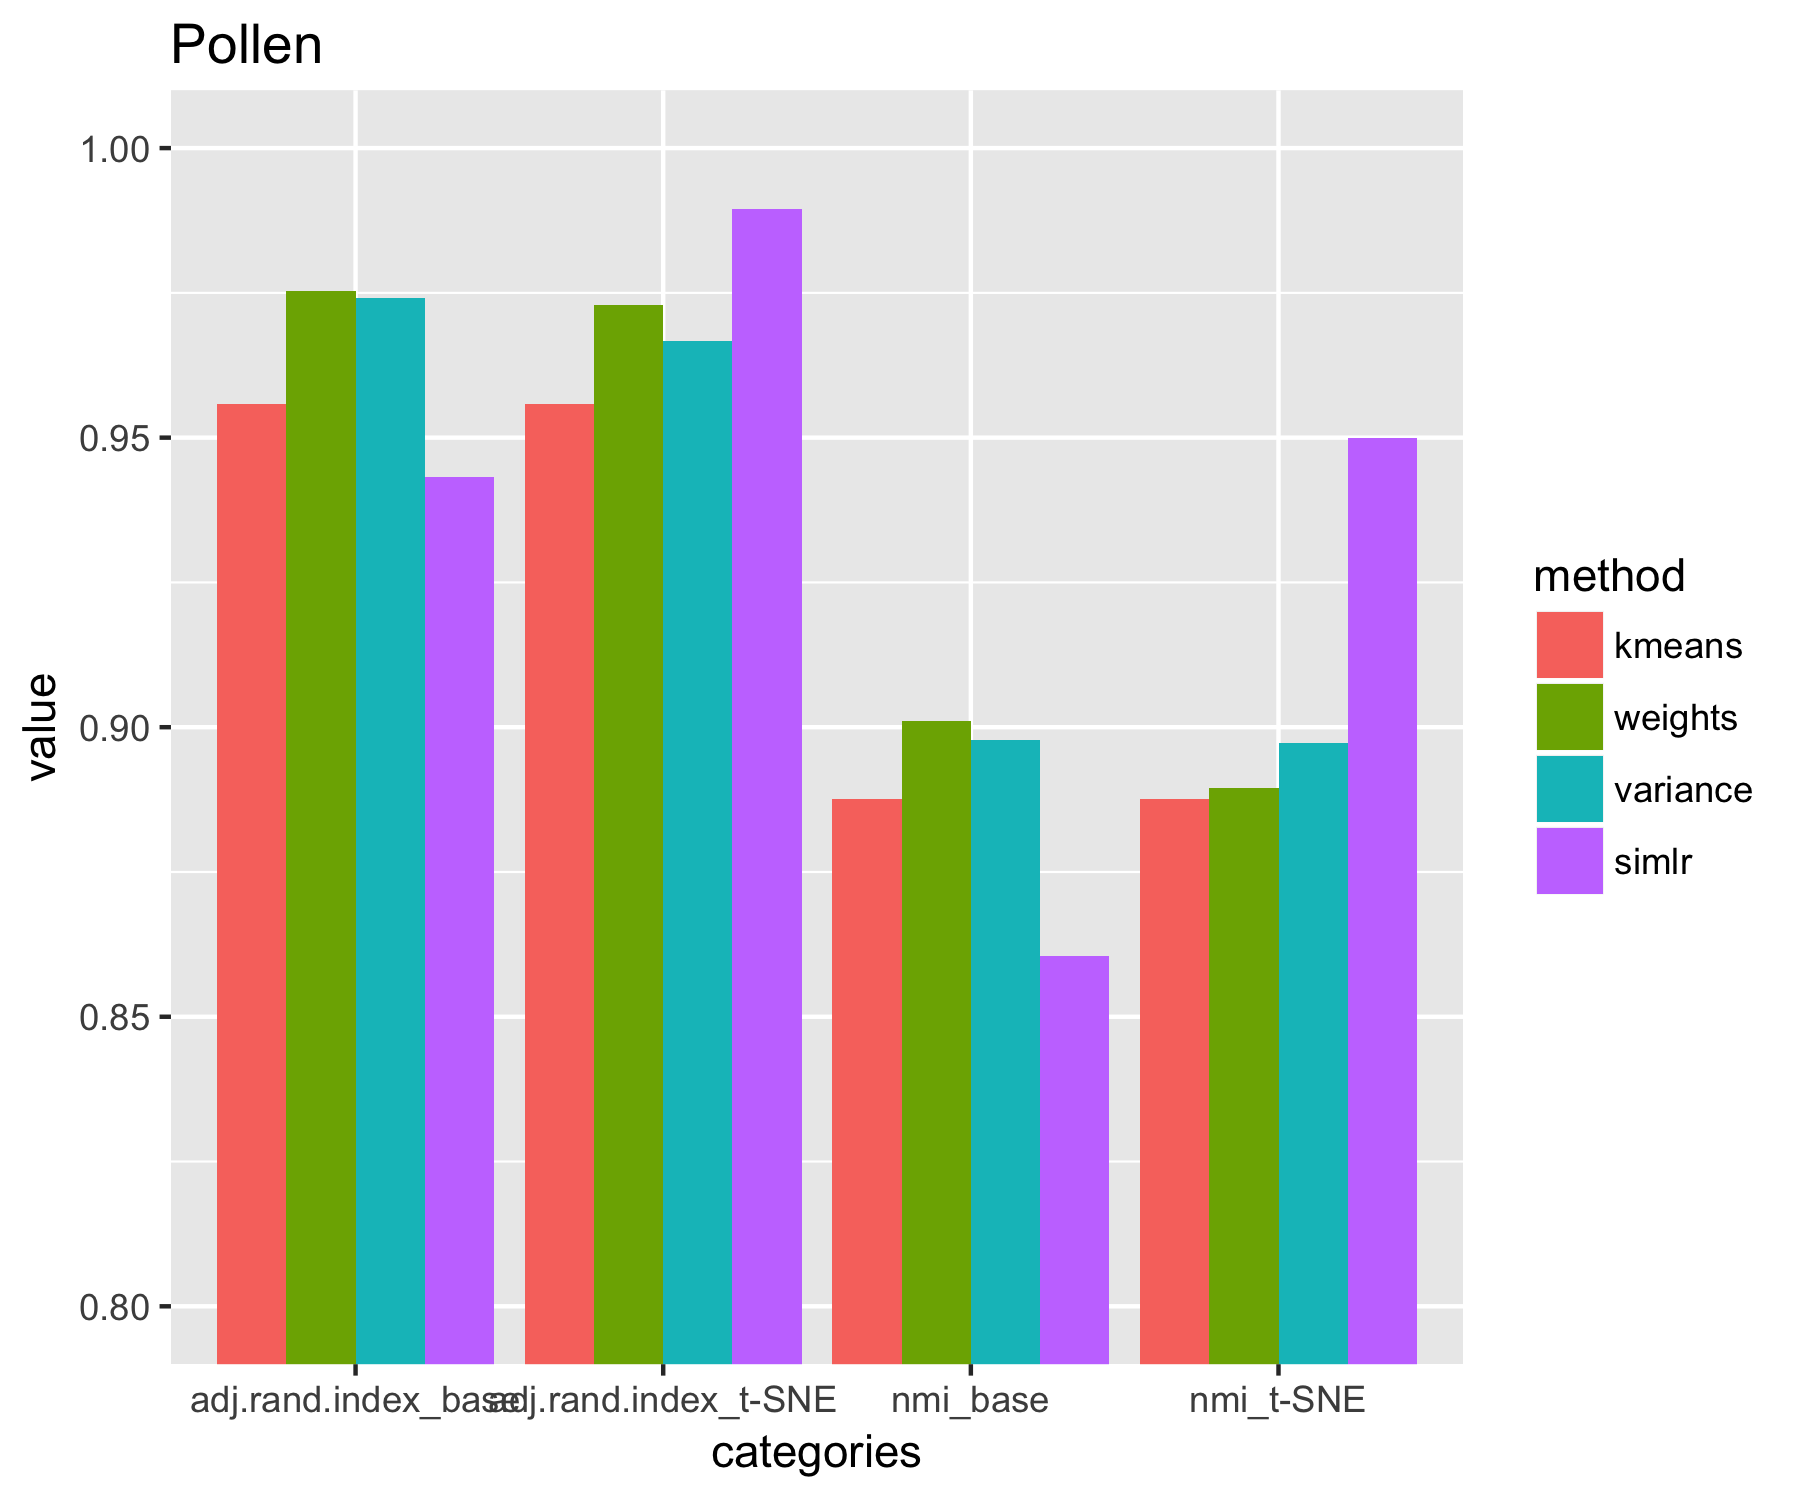
\includegraphics[width=0.45\linewidth]{Pollen_performance.png}\\
%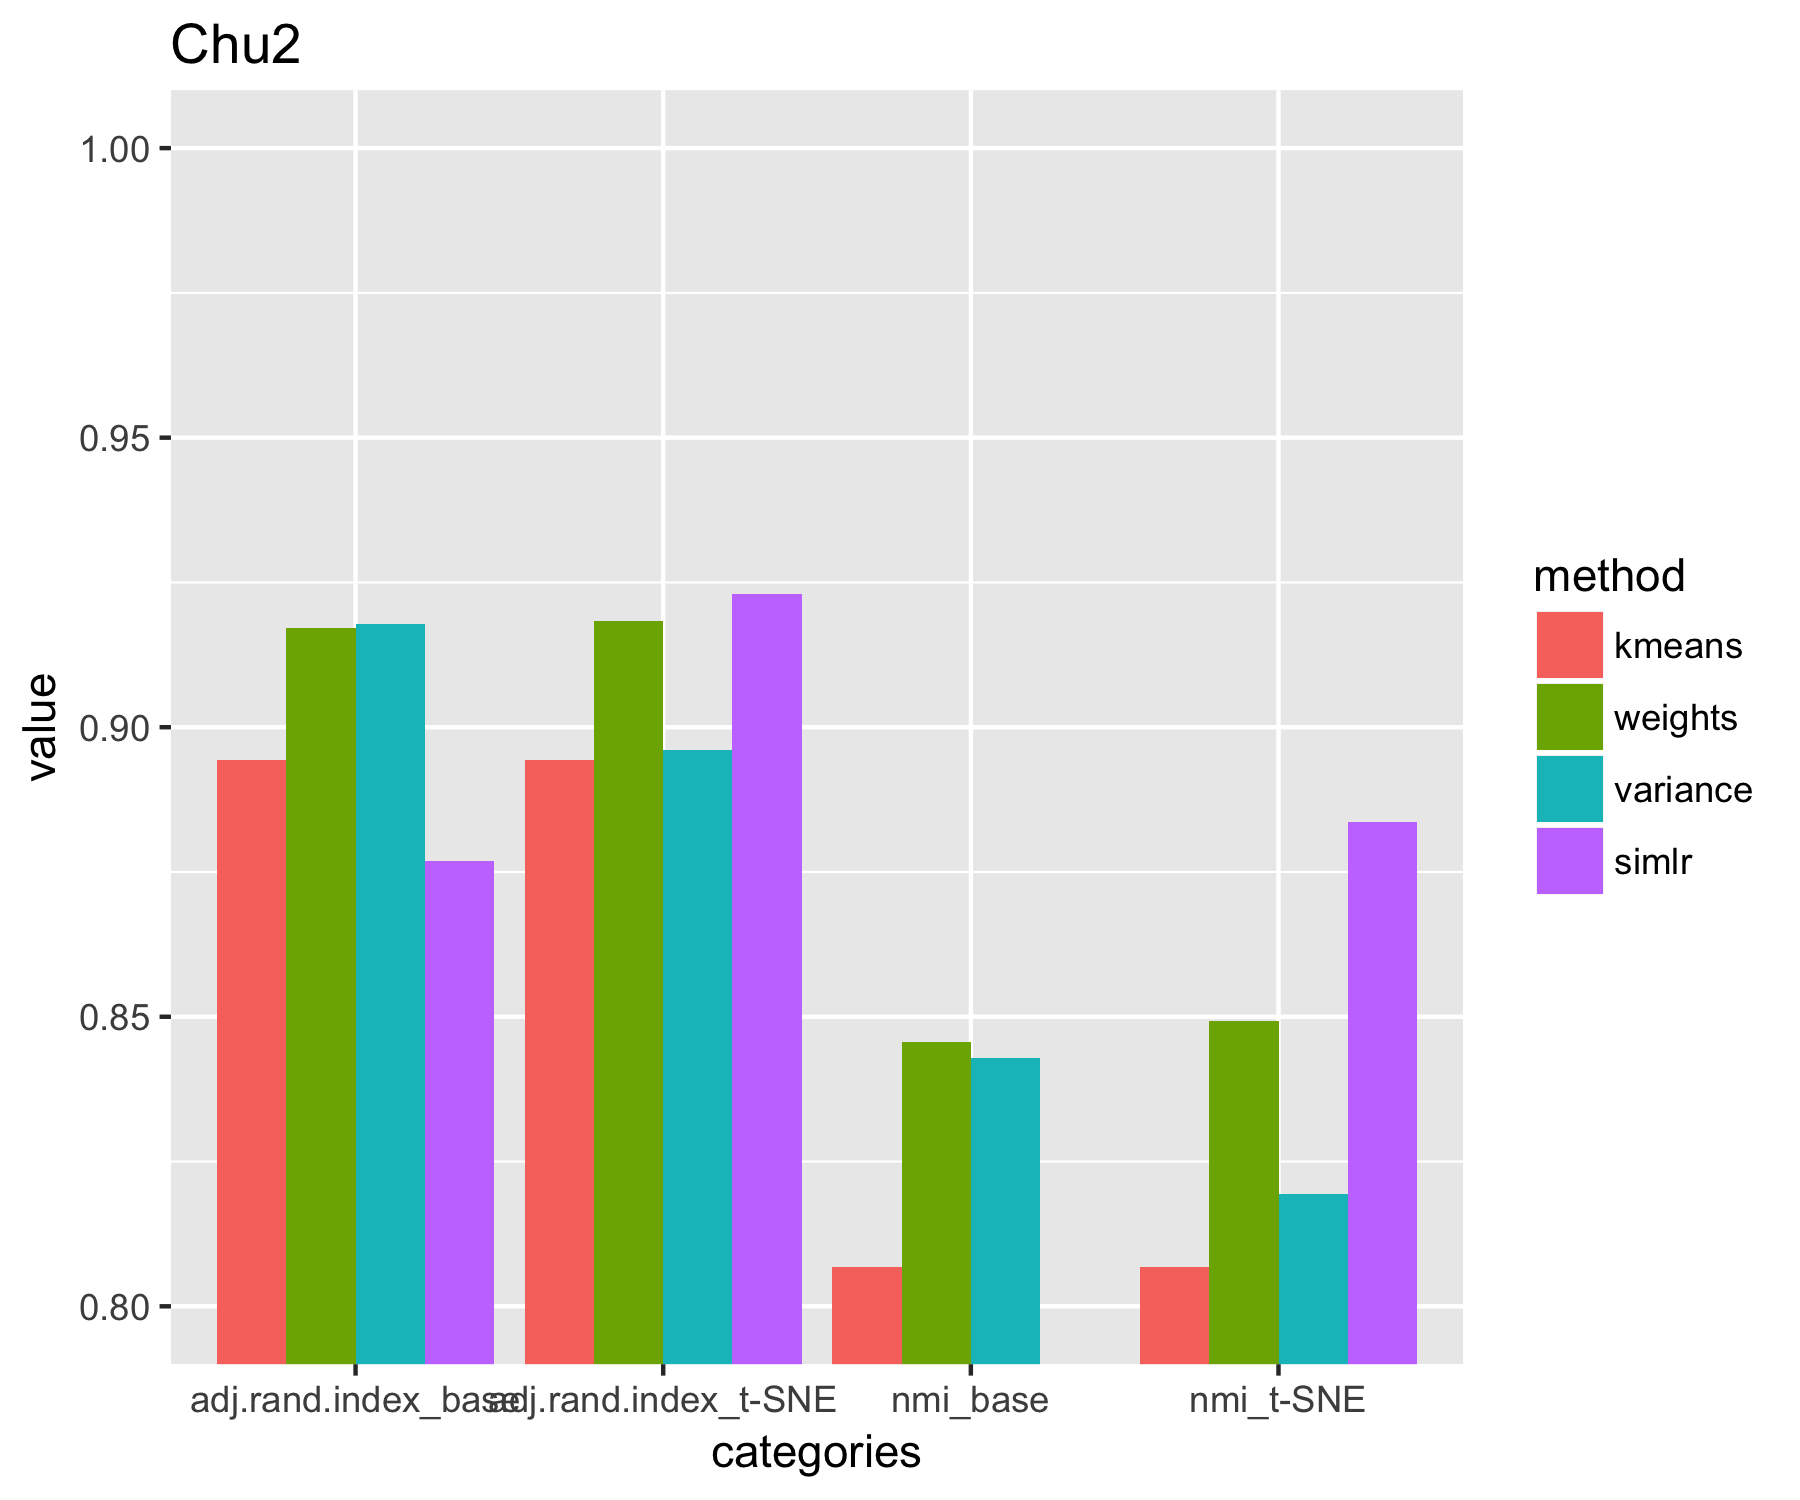
\includegraphics[width=0.45\linewidth]{Chu1_performance.png}
%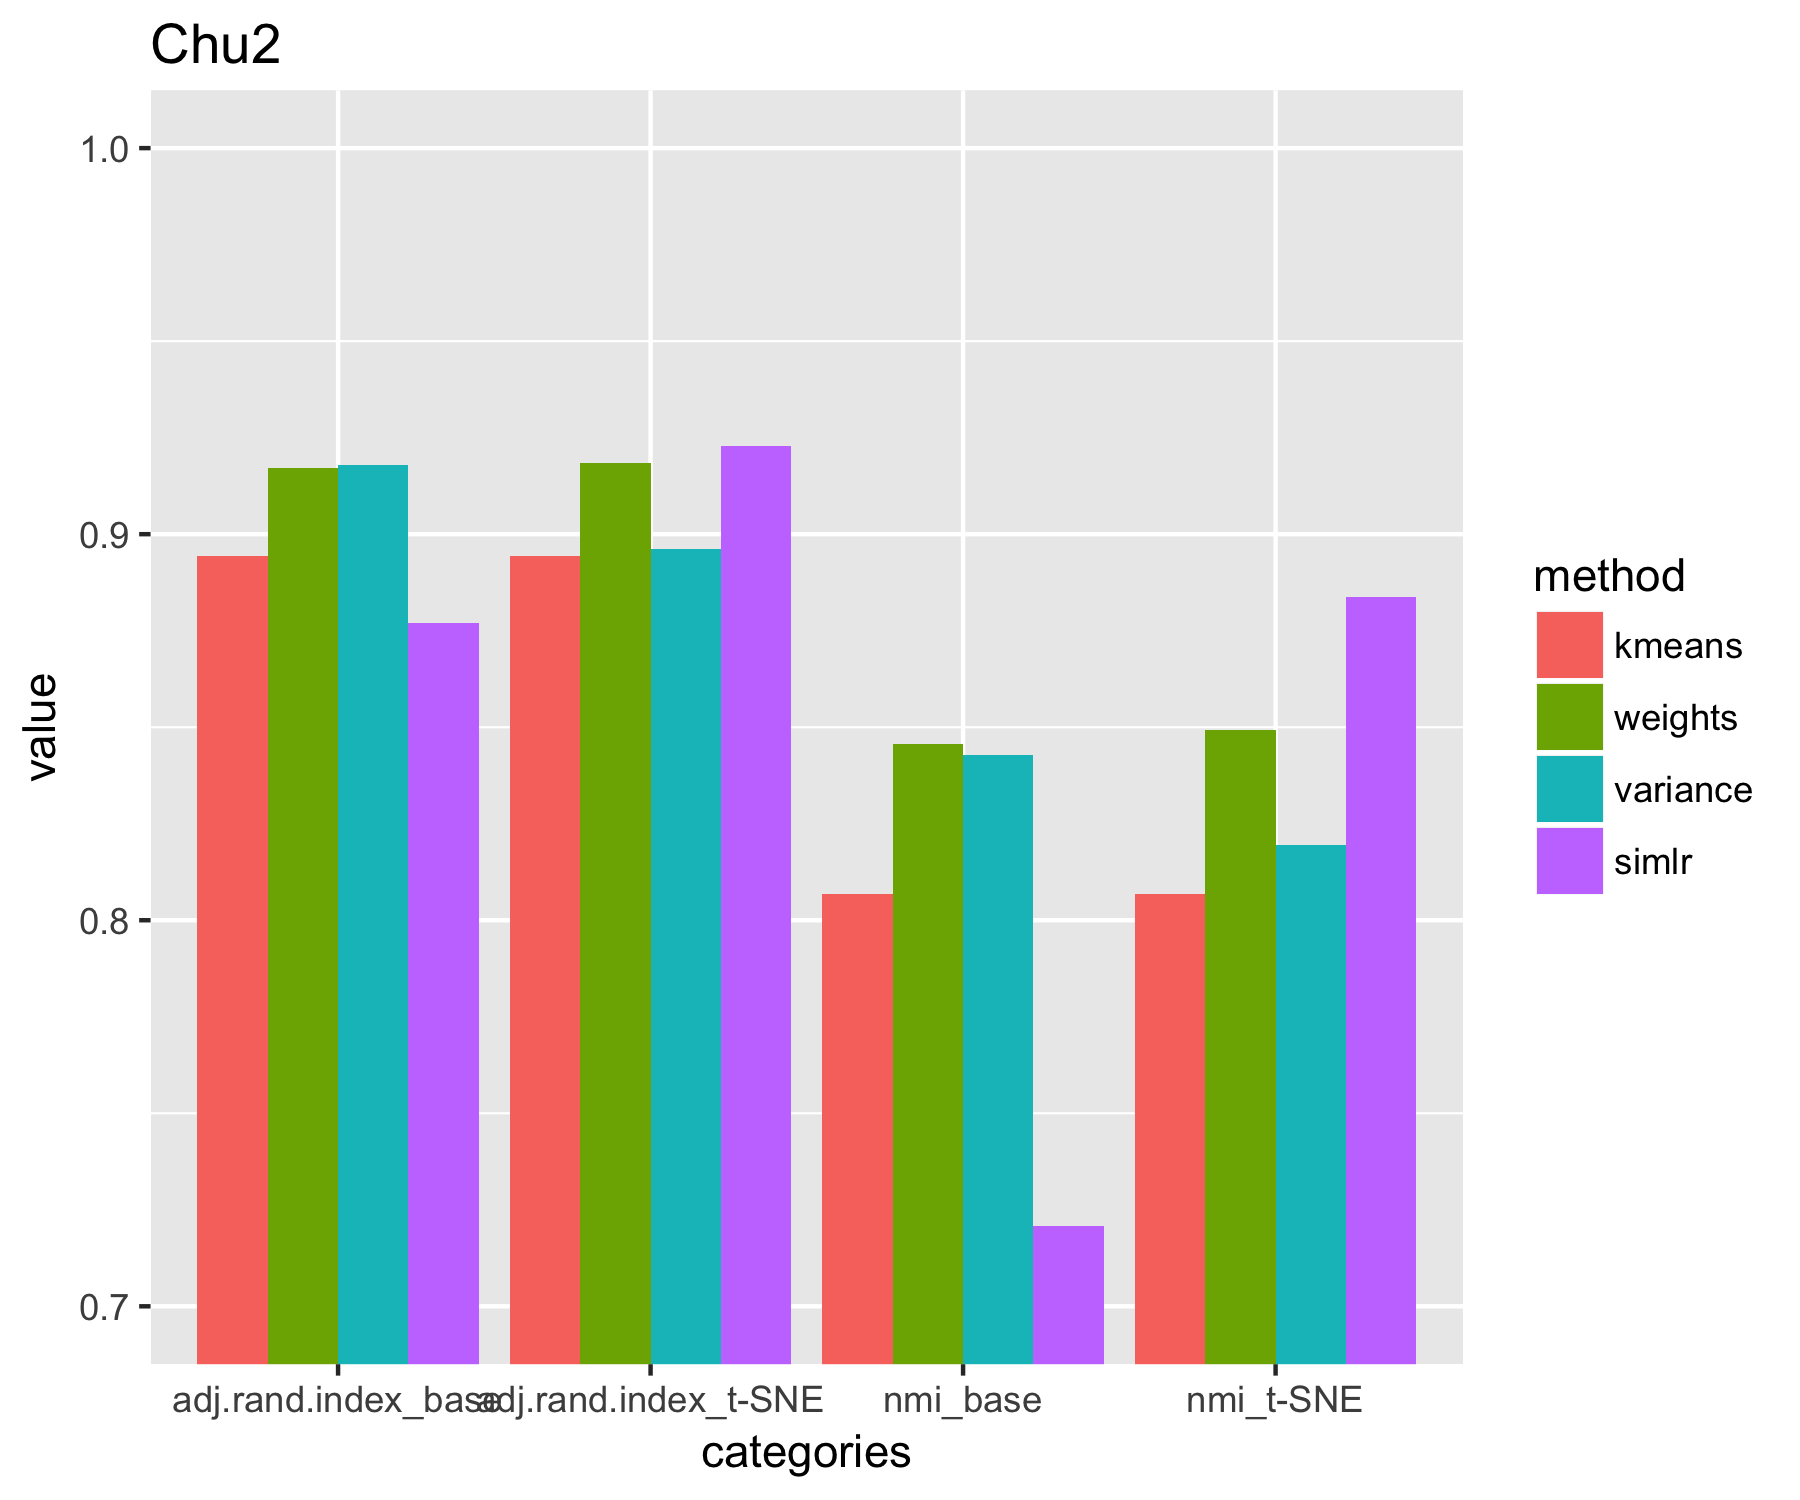
\includegraphics[width=0.45\linewidth]{Chu2_performance.png}
%\end{figure}


%\begin{center}
%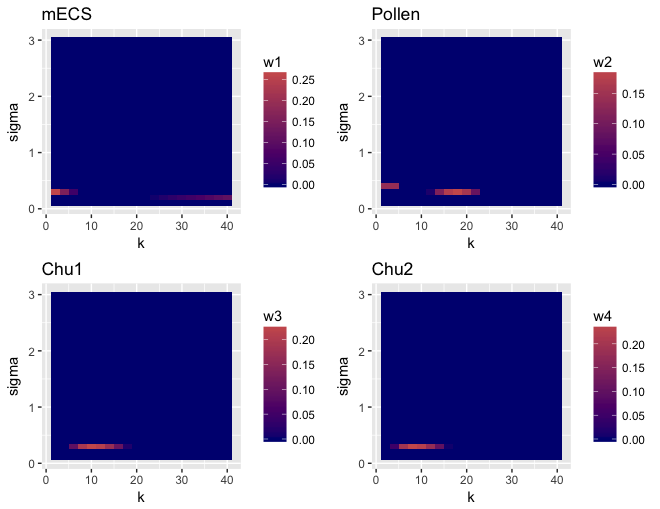
\includegraphics[width=0.7\linewidth]{w_kernel_selection.png}\\
%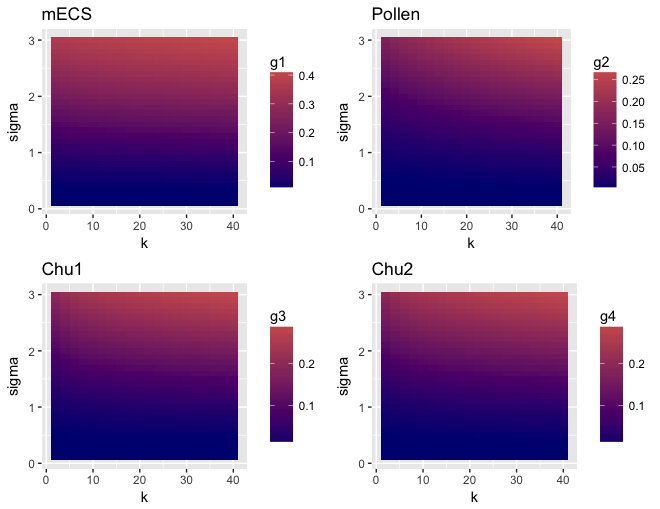
\includegraphics[width=0.7\linewidth]{g_kernel_selection.png}\\
%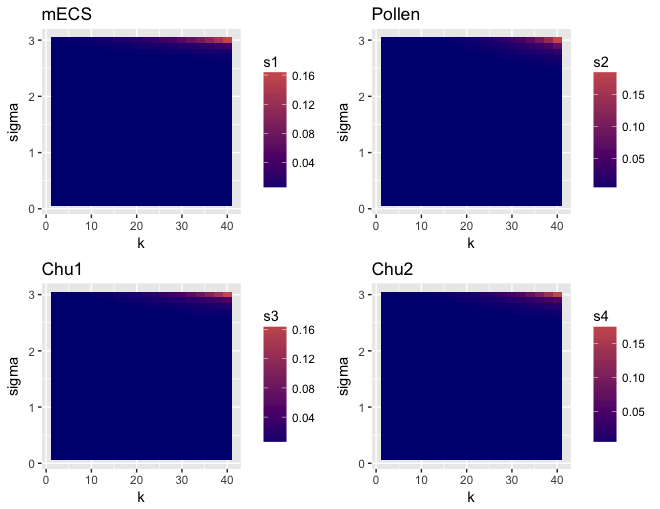
\includegraphics[width=0.7\linewidth]{s_kernel_selection.png}
%\end{center}
%
\begin{figure}[h]
\centering
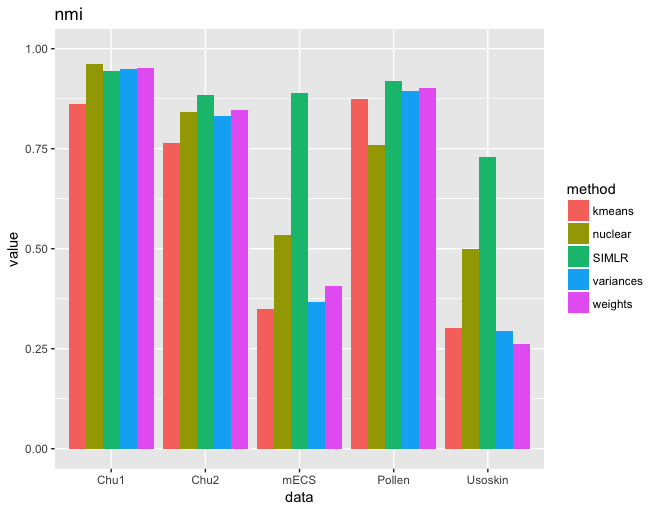
\includegraphics[width=0.45\linewidth]{nmi3.png}
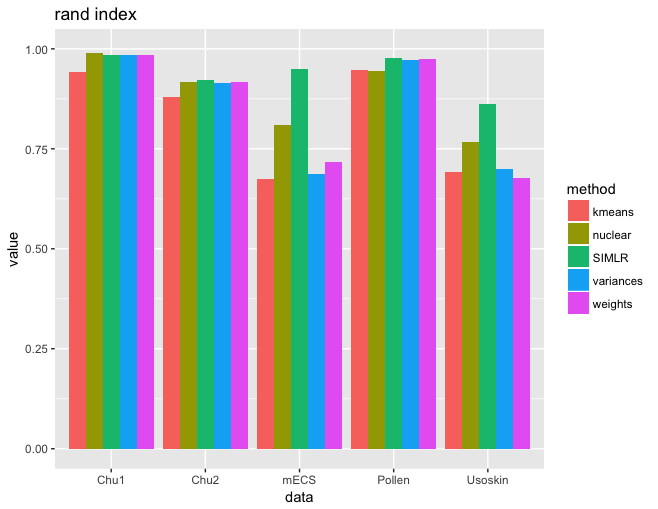
\includegraphics[width=0.45\linewidth]{ri3.png}
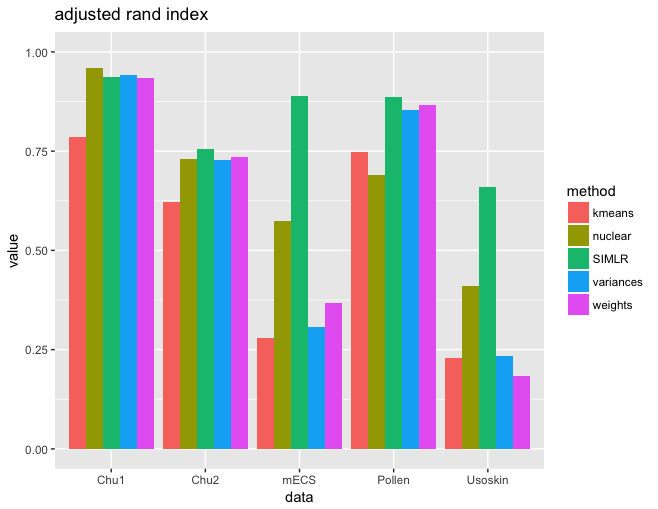
\includegraphics[width=0.45\linewidth]{ari3.png}
\end{figure}


%\section*{Model 4 : Re-introduce sparsity constraint}
%\subsection*{Objective 1 with sparsity}
%$$\arg \min_{S, w, c} \sum_{i=1}^{m} w_i \|P^{(i)}-S\|_F^2 + \sum_{i=1}^{m}w_i^2 + \sum_{i=1}^{m} c_i \| P^{(i)}-S\|_1 + \sum_{i=1}^{m} c_i^2$$
%where $P^{(i)} = S + E^{(i)}, S \geq 0, S\bm{1} = \bm{1}$
%Using new notation,
%$$\argmin_{S, E^{(i)}, w, c} w_i \|E^{(i)}\|_F^2 + c_i \|E^{(i)}\|_1 + \sum_{i=1}^{m} w_i^2 + \sum_{i=1}^{m} c_i^2$$
%Using Augmented Lagrangian,
%$$\mathcal{L}(S,E,w,c) = \sum_{i=1}^{m} w_i \|E^{(i)}\|_F^2 + c_i \|E^{(i)}\|_1 + w_i^2 + c_i^2 +\langle Y^{(i)}, S+E^{(i)}-P^{(i)}\rangle  + \frac{\mu}{2} \|S+E^{(i)}-P^{(i)}\|_F^2$$
%
%\begin{itemize}
%\item \textbf{update S}
%\begin{align*}
%\mathcal{L}(S) &= tr(Y^{(i)T}S) + \frac{\mu}{2} tr(S^TS + 2S^T(E^{(i)}-P^{(i)}))\\
%&= \frac{\mu}{2} tr(S^TS + 2(E^{(i)}-P^{(i)} + \frac{Y^{(i)}}{\mu})^T S)\\
%&= \frac{\mu}{2} \norm{S - \left(P^{(i)}-E^{(i)} - \frac{Y^{(i)}}{\mu}\right)}_F^2
%\end{align*}
%such that $rank(S) \leq r$. Do singular value decomposition of $\left( P^{(i)}-E^{(i)}-\frac{Y^{(i)}}{\mu}\right)$ and truncate the singular values after the first $r$.
%\item \textbf{update $E^{(i)}$}
%\begin{align*}
%\mathcal{L}(E^{(i)}) &= w_i tr(E^{(i)T}E^{(i)} + c_i \|E^{(i)}\|_1 + tr(Y^{(i)T}E^{(i)}) + \frac{\mu}{2} tr(E^{(i)T}E^{(i)} + 2E^{(i)T}(S-P^{(i)}))\\
%&= tr \left(
%\frac{2w_i+\mu}{2} E^{(i)T}E^{(i)} +\left(Y^{(i)} + \frac{\mu}{2} \cdot 2(S-P^{(i)})\right)^TE^{(i)}
%\right) + c_i \|E^{(i)}\|_1\\
%&= \frac{2w_i + \mu}{2} tr\left(E^{(i)T}E^{(i)} + \frac{2}{2w_i+\mu} (Y^{(i)} + \mu(S-P^{(i)})E^{(i)})\right) + c_i \|E^{(i)}\|_1\\
%&= \frac{2w_i + \mu}{2}\norm{
%E^{(i)} - \frac{\mu}{2w_i + \mu} \left(\frac{Y^{(i)}}{\mu} + S-P^{(i)} \right)
%}_F^2 + c_i \|E^{(i)}\|_1
%\end{align*}
%Then we can use soft thresholding to get a sparse $E^{(i)}$ : 
%$$E^{(i)} = S_{c_i / (2w_i +\mu)} \left( \frac{Y^{(i)}}{\mu} + S-P^{(i)}\right)$$
%\item \textbf{update $w_i$}
%$$\mathcal{L}(w_i) = \sum_{i=1}^{m} w_i^2 + w_i \|E^{(i)}\|_F^2$$
%$$\sum_{i=1}^{m} w_i = 1, w_i \geq 0$$
%We can use quadratic programming.
%\item \textbf{update $c_i$}
%$$\mathcal{L}(c_i) = \sum_{i=1}^{m} c_i^2 + c_i \|E^{(i)}\|_1$$
%$$\sum_{i=1}^{m} c_i = 1, c_i \geq 0$$
%We can use quadratic programming.
%\item \textbf{update $Y^{(i)}$}
%$$Y^{(i)} = Y^{(i)} + \mu (S+E^{(i)}-P^{(i)})$$
%\item \textbf{update $\mu$}
%$$\mu = \min(\mu \rho, \mu_{max})$$
%$\rho$ is a user-specified multiplier, $1.9$ by default.
%\end{itemize}
%
%\clearpage


%\section*{Understanding the Kernel}
%\begin{itemize}
%\item \textbf{Robust face recognition under partial occlusion based on support vector
%machine with local Gaussian summation kernel - Kazuhiro Hotta}\\
%$$K_p(x(p), y(p)) = exp \left(
%-\frac{\|x(p)-y(p)\|^2}{\sigma_p^2}
%\right)$$
%where $p$ is the label of position and $x(p)$ and $y(p)$ are the local features centered at position $p$. $\sigma_p^2$ is the local variance at position $p$. The paper's interest is in SVM and so their conclusion is that the optimal hyperplane is
%$$f(x) = \sum_{i \in SV} \alpha_i y_i \frac{1}{N} \sum_{p}^{N} exp \left(
%-\frac{\|x(p)-y(p)\|^2}{\sigma_p^2}
%\right) + b$$
%but this is not what we care about.
%
%\item \textbf{Adaptive spherical Gaussian kernel in sparse Bayesian learning framework for nonlinear regression - JinYuan, LiefengBo, KeshengWang, TaoYu}\\
%\noindent They define four kernels. 
%$$k_0(X_m, X) = exp \left(
%-\sum_{d=1}^{D} \frac{\|x_m^{(d)} - x^{(d)}\|^2}{2\ell^2}
% \right)$$
% $$k_1(X_m, X) = exp \left(
% -\sum_{d=1}^{D} \frac{\|x_m^{(d)} - x^{(d)}\|^2}{2\ell_d^2}
% \right)$$
% $$k_2(X_m, X) = exp \left(
% -\sum_{d=1}^{D} \frac{\|x_m^{(d)} - x^{(d)}\|^2}{2\ell_m^2}
% \right)$$
% $$k_3(X_m, X) = exp \left(
% -\sum_{d=1}^{D} \frac{\|x_m^{(d)} - x^{(d)}\|^2}{2\ell_{md}^2}
% \right)$$ 
% $\mathbb{R}^D$ is the input space for the features. $k_1$ is variant to the features but not to the number of $SV = M$. $k_2$ is variant to the SV's but not to the features. $k_3$ is the most flexible kernel that is adaptive to both SV and features, but computational burden is too high and it leads to easier overfitting.
% 
%\item \textbf{Similarity network fusion for aggregating data types on a genomic scale - Anna Goldenberg}\\
%
%\noindent $n$ samples, $m$ measurements. A patient similarity network is represented as a graph $G=(V,E)$. The edge weights are represented by $n \times n$ similarity matrix $W$. $\rho(x_i, x_j)$ is a Euclidean distance between patients $x_i$ and $x_j$. First, let's define the weight of the edge as
%$$W(i,j) = exp \left( -\frac{\rho^2(x_i, x_j)}{\mu \epsilon_{ij}}\right)$$
%\noindent where $\mu$ is a hyperparameter that can be empirically set and $\epsilon_{ij}$ is used to eliminate the scaling problem. 
%$$\epsilon_{ij} = \frac{\text{mean}(\rho(x_i, N_i)) + \text{mean}(\rho(x_j,N_j)) + \rho(x_i,x_j)}{3}$$
%\noindent To compute this kernel, build a sparse kernel and a full kernel. The full kernel is a normalized weight matrix $P = D^{-1}W$. $D$ is the diagonal degree matrix. However, this suffers from numerical instability since it involves self-similarities on the diagonal entries. A better normalization is
%$$P(i,j) = \frac{W(i,j)}{2\sum_{ k \neq i} W(i,k)}$$
%for $j \neq i$ and $P(i,j)  = \frac{1}{2}$ otherwise. This normalization keeps the $P \bm{1} = \bm{1}$
%The local affinity, meanwhile, is defined like this:
%$$S(i,j) = \frac{W(i,j)}{\sum_{k \in N_i} W(i,k)}$$
%if $j \in N_i$ and 0 otherwise. In other words, this operation sets the similarities between non-neighboring points to zero using KNN. We are making the assumption that local similarities are more reliable than remote ones. 
%\end{itemize}


%
%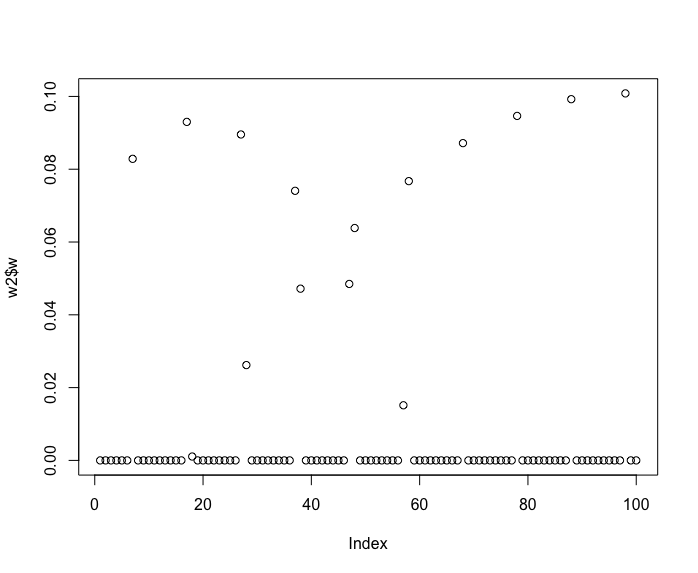
\includegraphics[width=0.45\linewidth]{weights.png}
%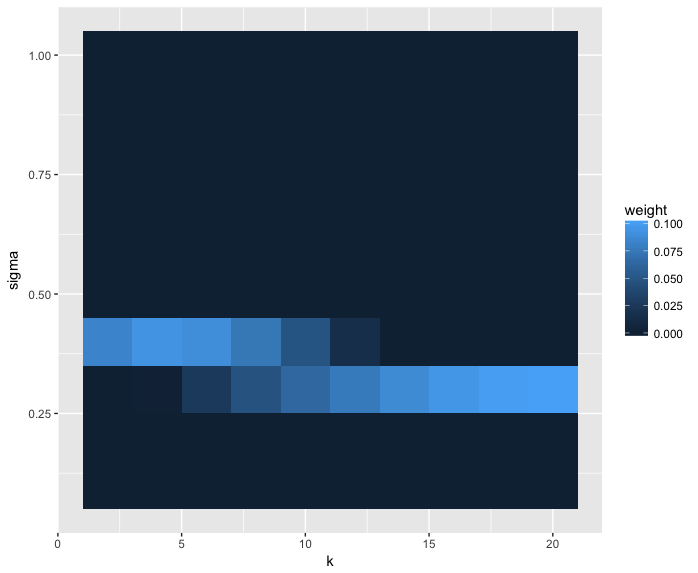
\includegraphics[width=0.45\linewidth]{weights2.png}
%
%\clearpage
%
%
%\begin{center}
%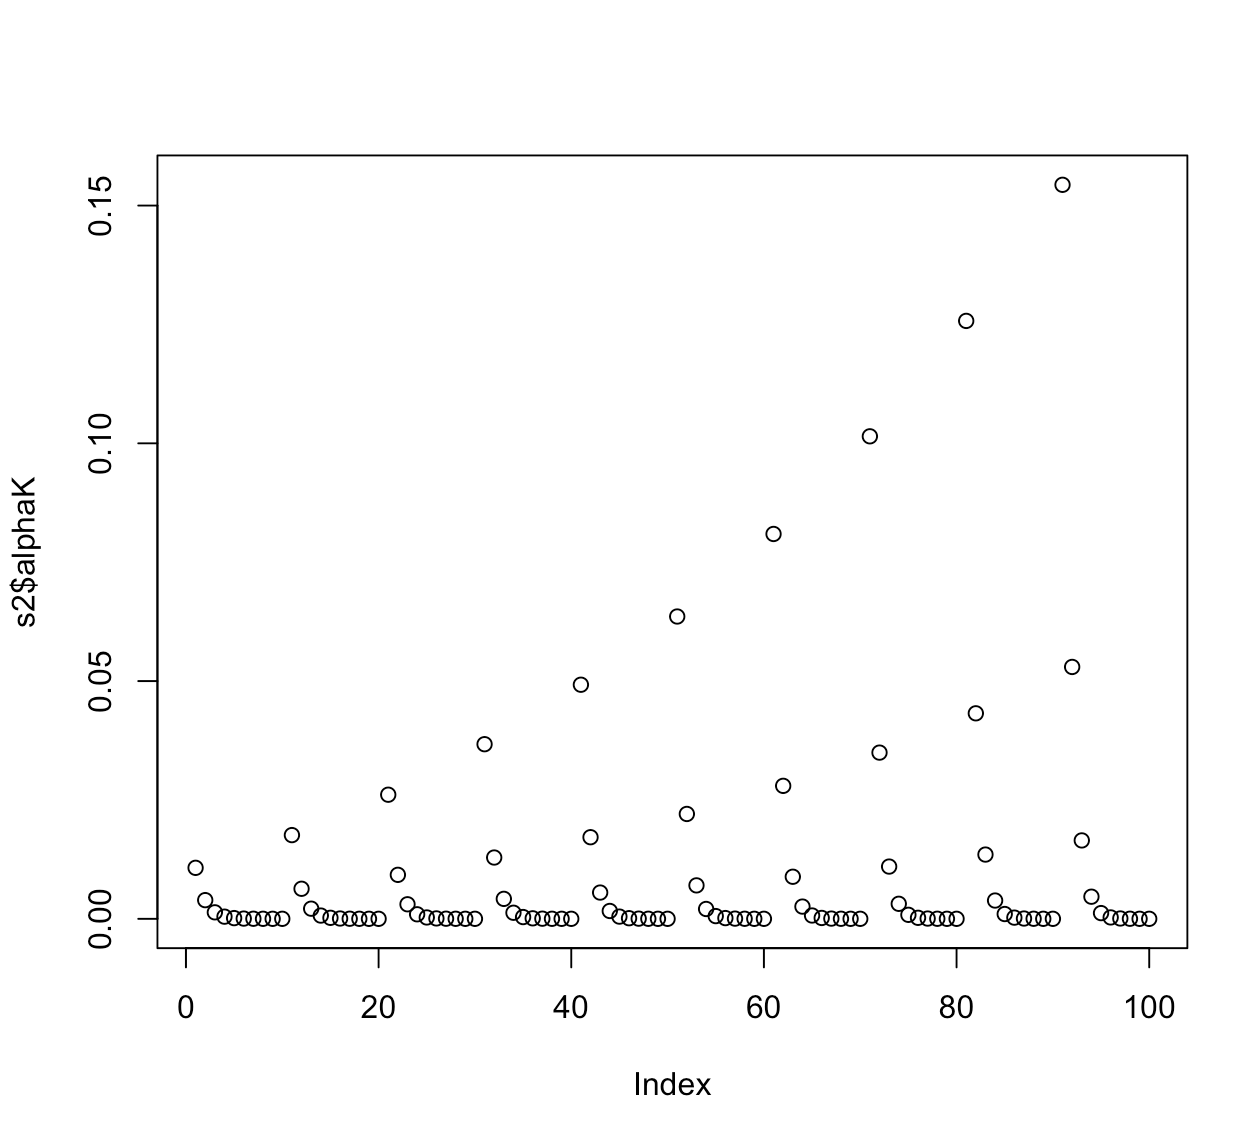
\includegraphics[width=0.45\linewidth]{SIMLR.png}
%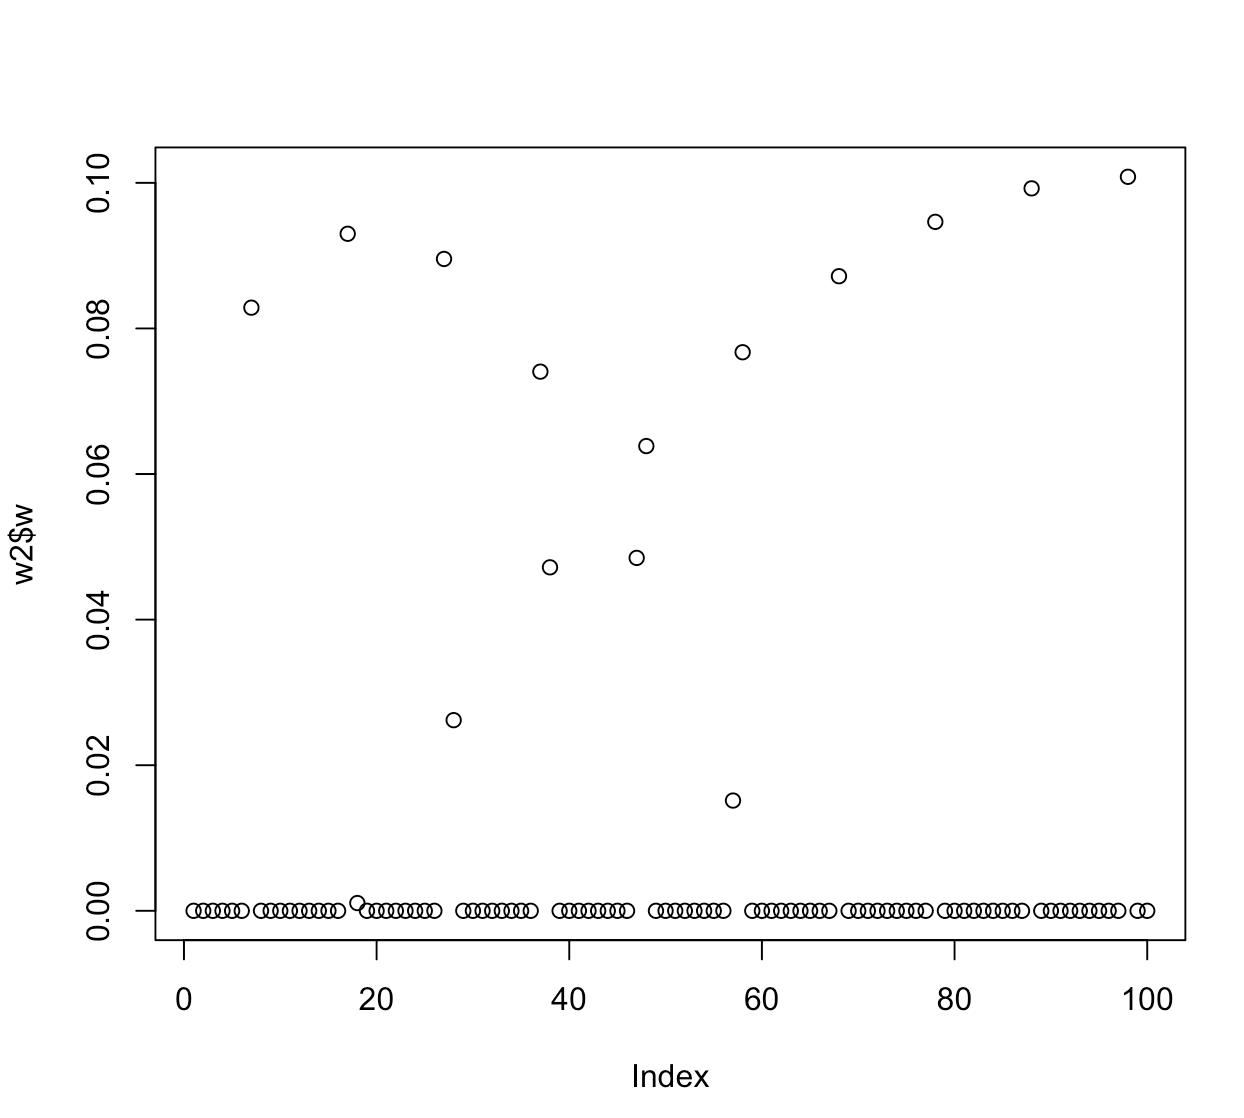
\includegraphics[width=0.45\linewidth]{weights23.png}
%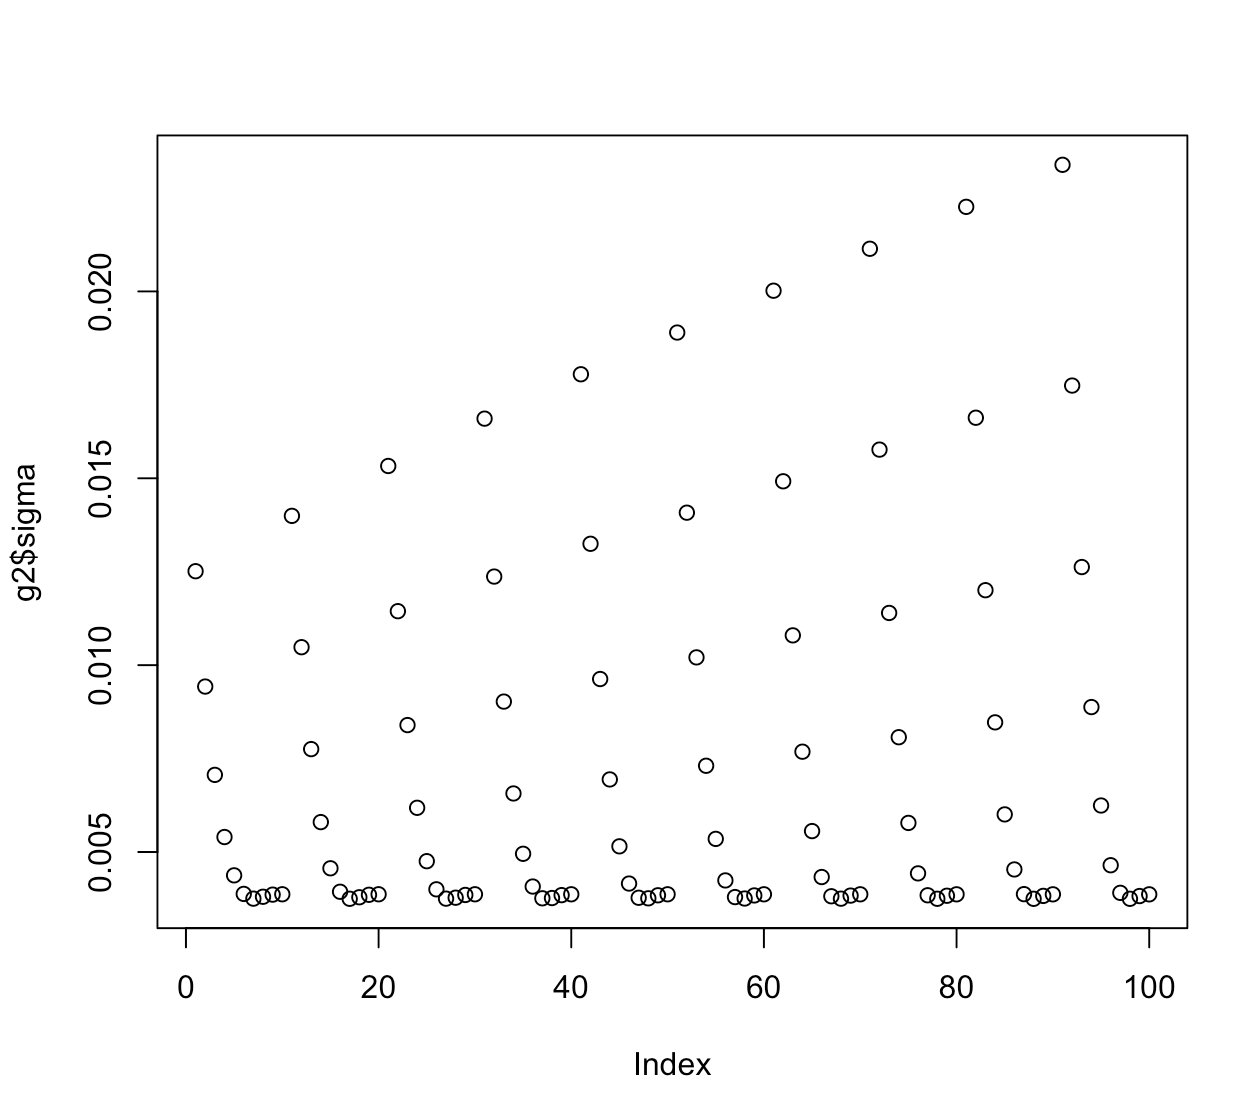
\includegraphics[width=0.45\linewidth]{sigma.png}

%\end{center}



\section*{Re-visit nuclear norm}
$$\min_S \sum_{i=1}^{m} w_i^2 \|S-P^{(i)}\|^2_F + \tau \|S\|_* \text{  such that  }S1 = 1, S\geq 0, \sum_i w_i = 1, w_i \geq 0$$
$$\mathcal{L} = \tau \|Q\|_* + \sum_{i=1}^{m} w_i \|Q-P^{(i)}\|_F^2 + \langle Y, S-Q \rangle + \frac{\mu}{2} \|S-Q\|_F^2 + \sum_i w_i^2$$

\begin{itemize}
\item \textbf{update Q}\\
$$\argmin_Q \tau \|Q\|_* + \sum_{i=1}^{m} \frac{w_i}{2} \|Q-P^{(i)}\|_F^2 + \langle Y, S-Q \rangle + \frac{\mu}{2} \|S-Q\|_F^2$$
$$=\argmin_Q \tau \|Q\|_*+ \frac{\mu+2}{2} \norm{Q - \frac{1}{(\mu+2)} \left(\sum_i w_i P_i + \mu S + Y\right)}_F^2$$
So we take SVD of $\frac{1}{\mu + 2} \left( \sum_i w_i P_i + \mu S + Y \right)$ and take the soft threshold on the singular values using $\frac{\tau}{\mu+2}$
\item \textbf{update S}\\
$$\argmin_S \norm{ S - \left( Q-\frac{Y}{\mu}\right)}_F^2$$
Therefore project onto the domain $S \geq 0$, $S1=1$ using $Q-\frac{Y}{\mu}$. 
\end{itemize}

\section*{Include rank information through Laplacian matrix}
$$\min_{S, J, w} \tau \|S\|_* + \gamma tr(J^T D^{-1/2} (I-S) D^{-1/2} J) + \frac{1}{2} \sum_i w_i \|S-P_i\|_F^2 + \frac{1}{2} \sum_i w_i^2$$
$$\mathcal{L}= \tau \|Q\|_* + \gamma tr(J^T D^{-1/2} (I-Q)D^{-1/2} J) + \frac{1}{2} \sum_i w_i \|Q-P_i\|_F^2 + \frac{1}{2} \sum_i w_i^2 + \langle Y, S-Q \rangle + \frac{\mu}{2} \|S-Q\|_F^2$$
\begin{itemize}
\item \textbf{update Q}
$$\argmin_Q \tau \|Q\|_* + \frac{\mu+1}{2} \|Q - \frac{1}{\mu+1} (\gamma \tilde{J} \tilde{J}^T + \sum_i w_i P_i + Y + \mu S) \|_F^2$$
Therefore, do the SVD of $\gamma \tilde{J} \tilde{J}^T + \sum_i w_i P_i + Y + \mu S$ and do the soft thresholding with $\frac{\tau}{\mu+1}$
\item \textbf{update S}
$$\argmin_S \frac{\mu}{2} \|S - (Q-\frac{Y}{\mu})\|_F^2$$
\item \textbf{update J}
$$\argmax_J tr(J^T D^{-1/2} (S-I) D^{-1/2} J)$$
So $J$ is the first $r$ eigenvalues of $D^{-1/2}(S-I) D^{-1/2}$

\end{itemize}


\clearpage

\section*{Record of Optimization Goals}
\subsection*{1. objective\_1\_c}
$$\min_{S,w} \frac{1}{2} \sum_{i=1}^{m} w_i \|S-P_i\|_F^2 + \sum_{i=1}^{m} w_i^2$$
$S1 = 1, S \geq 0, rank(S) \leq r, w \geq 0, \sum_{i=1}^{m} w_i = 1$
\subsection*{2. objective\_2\_c}
$$\min_{S,\sigma} \sum_{i=1}^{m} \frac{\|S-P_i\|_F^2}{2n^2 \sigma_i} + \frac{\sigma_i}{2}$$
$S1 = 1, S\geq 0, rank(S) \leq r$
\subsection*{3. objective\_3}
$$\min_{S,w} \sum_{i=1}^{m} w_i \|S-P_i\|_F^2 + \tau \|S\|_* + \frac{1}{2} \sum_i w_i^2$$
$S1 = 1, S\geq 0, \sum w_i = 1, w \geq 0$
\subsection*{4. objective\_4}
$$\min_{S,J,w} \sum_{i=1}^{m} w_i \|S-P_i\|_F^2 + \tau \|S\|_* + \gamma tr(J^T \tilde{L} J)+ \frac{1}{2} \sum_i w_i^2$$
$S1 = 1, S\geq 0, \sum w_i = 1, w \geq 0$
\subsection*{5. objective\_5}
$$\min_{S,J,w} \sum_{i=1}^{m} w_i \|S-P_i\|_F^2 + \tau \|S\|_* + \gamma tr(J^T \tilde{L} J)+\gamma \|S\|_F^2 + \frac{1}{2} \sum_i w_i^2$$
$S1 = 1, S\geq 0, \sum w_i = 1, w \geq 0, J^TJ = I_r$
\noindent Note that it's equivalent to
$$\min_{S,J,w} \sum_{i=1}^{m} w_i \|S-P_i\|_F^2 + \tau \|S\|_* + \gamma \|S - \frac{1}{2} JJ^T \|_F^2 + \frac{1}{2} \sum_i w_i^2$$
with the same constraints. An extra penalty term is pushing $S$ towards rank $r$ matrix $JJ^T$. 
\subsection*{6. obectjve\_6}
$$\min_{S} \sum_i w_i \|S-P_i\|_F^2 + \sum_i w_i^2$$
$S1 = 1, S\geq 0, \sum w_i = 1, w \geq 0, rank(L_S) = n-k$
\subsection*{7. nuclear\_scaledlasso}
$$\min_{S,w} \sum_{i=1}^{m} \frac{\|S-P_i\|_F^2}{2n^2 \sigma_i} + \tau \|S\|_* + \frac{1}{2} \sum_i \frac{\sigma_i}{2}$$
$S1 = 1, S\geq 0$
\subsection*{8. Laplacian1}
$$\tau \|I - L\|_* + \sum_i \frac{\|L-M_i\|_F^2}{2n^2 \sigma_i} + \sum_i \frac{\sigma_i}{2}$$
$L$ is the true Laplacian matrix, $M_i$ is the $i$'th observed Laplacian matrix. We use \textbf{unnormalized} similarity matrix to construct Laplacian so that the use of row sums when constructing the Laplacian accounts for the local structure. 
\subsection*{9. Laplacian2}
$$\tau \|I - L\|_* + \sum_i w_i \|L-M_i\|_F^2 + \sum_i w_i^2$$
$w_i \geq 0$, $\sum_i w_i = 0$
Same as above except that weight is used instead of scaled lasso.


\pagebreak

%\noindent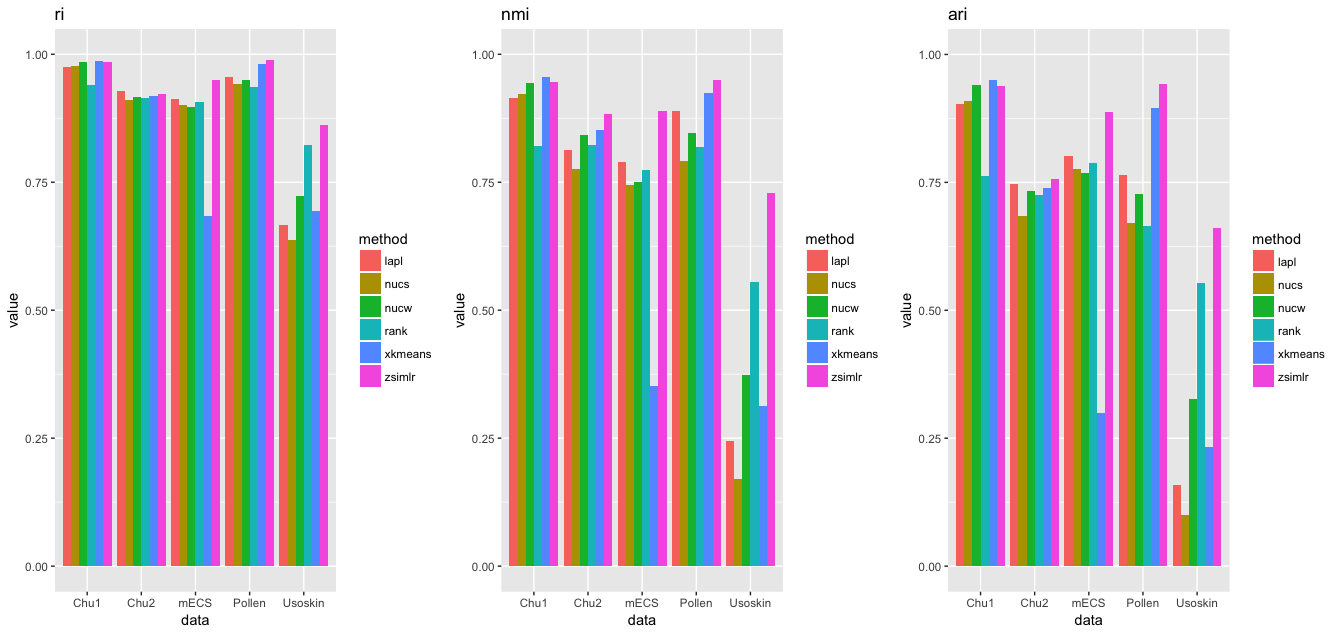
\includegraphics[width=0.98\linewidth]{mysterykernel_performance.png}
%\noindent 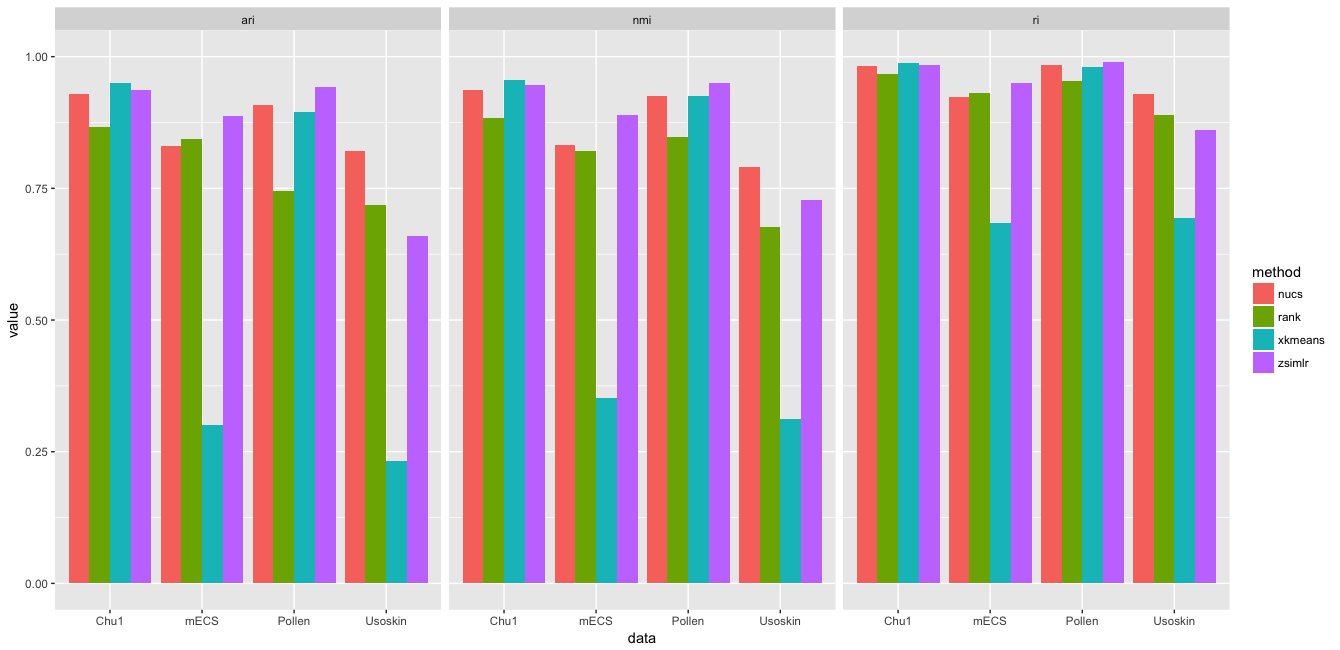
\includegraphics[width=0.98\linewidth]{different_initial1.png}
\begin{itemize}
\item \textbf{nucs}
$$\min_{S,w} \sum_{i=1}^{m} \frac{\|S-P_i\|_F^2}{2n^2 \sigma_i} + \tau \|S\|_* + \frac{1}{2} \sum_i \frac{\sigma_i}{2}$$
$S1 = 1, S\geq 0$
\item \textbf{rank}
$$\min_{S,J,w} \sum_{i=1}^{m} w_i \|S-P_i\|_F^2 + \tau \|S\|_* + \gamma tr(J^T \tilde{L} J)+ \frac{1}{2} \sum_i w_i^2$$
$S1 = 1, S\geq 0, \sum w_i = 1, w \geq 0$
\item \textbf{kmeans}
Kmeans on the entire feature set

\item \textbf{zsimlr}
Software SIMLR with its default initialization
\end{itemize}


\pagebreak

\section*{Initialization: how to build $P$}
\begin{itemize}
\item \textbf{Build similarity matrices $K_{\ell}$ with different kernel parameters}\\
Start with data matrix $X \in \mathbb{R}^{n \times p}$ where $n$ is the number of cells and $p$ is the number of features. First, build Euclidean distance matrix $D \in \mathbb{R}^{n \times n}$ where
$$D_{ij} = \|x_i - x_j\|_2^2$$
$x_i$ and $x_j$ are cells $i$ and $j$ taken from the $i$'th and $j$'th rows of $X$.  Since we are using multiple kernels with different sets of parameters, use index $\ell \in \{ 1, 2, \cdots , L\}$ to denote that the kernel is built with parameters$k_{\ell}$ and $\sigma_{\ell}$. The default initialization is $k_{\ell}\in \{10,15,20,25,30\}$ and $\sigma_{\ell} \in \{2,1.9,1.8,1.7,1.6,1.5,1.4,1.3,1.2,1.1,1\}$. Now, for each $\ell$, build $\mu_{\ell} \in \mathbb{R}^{n \times 1}$ vector that averages the distance to $k$ nearest neighbors.
$$\mu_{i\ell} = \frac{\sum_{j \in KNN_{\ell} (x_i)}\|x_i - x_j\|_2^2}{k_{\ell}}$$
Now we can build the variance matrix $\epsilon_{\ell}$:
$$\epsilon_{i,j,\ell} = \frac{(\mu_i + \mu_j)\sigma_{\ell}}{2}$$
$\mu$ and $\epsilon$ account for the local structure. If two nodes are relatively isolated from other nodes, the distance between them is adjusted to be smaller. Finally, we use $\epsilon_{\ell}$ to build the similarity matrix $K_{\ell} \in \mathbb{R}^{n \times n}$:
$$K_{i,j,\ell} = N(D_{ij}; 0, \epsilon_{i,j,\ell})$$
$$= \frac{1}{\sqrt{2\pi}\hspace{1mm} \epsilon_{i,j,\ell}} exp \left( 
-\frac{D_{ij}}{2\epsilon_{i,j,\ell}^2}
\right)$$

\item \textbf{Build normalized distance matrix $C$}\\
Build distance matrix $C$ that again adjusts for the local structure:
$$C_{i,j,\ell} = K_{i,i,\ell} + K_{j,j,\ell} - 2K_{i,j,\ell}$$

\item \textbf{Using knn, build sparse similarity matrices $P$}\\
For each $\ell$ (dropping the subscript $\ell$ in this section), only take the closest $k+1$ neighbors' distances and indices using $C$ and build two matrices
$$M, I \in \mathbb{R}^{n \times (k+1)}$$
The $i$'th row of matrix $M$ has an ordered distance for point $i$'s $k+1$ nearest neighbors, and $I$ has the corresponding indices of those neighbors. Then, convert this back to a similarity matrix by subtracting each column from the $(k+1)$'th column of $M$ so that the $(k+1)$'th column becomes a vector of 0's. Removing this last column, now we have $\tilde{M} \in \mathbb{R}^{n \times k}$ that has the largest similarity in the first column and the smallest similarity in the $k$'th column. Then normalize $\tilde{M}$ so that each row sums to 1. The similarity measures are all 0's except these $k$ nearest neighbors. Now create similarity matrix $A$ by assigning these nonnegative similarity measures to its correct indices of the neighbors. Now, $A \in \mathbb{R}^{n \times n}$ is a transition probability matrix that is element-wise non-negative and has row sums of 1. Then finally create symmetric similarity matrix $P$ from $A$.
$$P = (A + A^T) / 2$$
\end{itemize}

\section*{Optimization algorithm}
%We solve the following to get the underlying true similarity matrix $S$.
%$$\min_{S,\sigma} \sum_{i=1}^{m} \frac{\|S-P_i\|_F^2}{2n^2 \sigma_i} + \tau \|S\|_* + \sum_i \frac{\sigma_i}{2}$$
%$S1 = 1, S\geq 0$.\\ 
%We employ the scaled lasso to give different weights to each observed similarity $P_i$ and to control the noise level simultaneously. 
%
%$$\mathcal{L} = \sum_{i=1}^{m} \frac{1}{2n^2 \sigma_i} \|Q-P_i\|_F^2 + \tau \|Q\|_* + \sum_i \frac{\sigma_i}{2} + \langle Y, S-Q \rangle + \frac{\mu}{2} \|S-Q\|_F^2$$
%\begin{itemize}
%\item \textbf{update $Q$}\\
%Defining $\phi = \mu + \sum_i \frac{1}{n^2 \sigma_i}$,
%$$\mathcal{L}(Q) = \frac{\phi}{2} \norm{Q - \frac{1}{\phi} \left( \sum_i \frac{P_i}{n^2 \sigma_i} + Y + \mu S\right) }_F^2$$
%Then soft-threshold the singular values of $Q$ by $\frac{\tau}{\phi}$
%\item \textbf{update $S$}
%$$\mathcal{L}(S) = \norm{S-\left(Q-\frac{Y}{\mu}\right)}_F^2$$
%where  $S\geq 0$ and $S1=1$
%\item \textbf{update $\sigma$}
%$$\sigma_i = \frac{\|P_i - Q\|_F^2}{n^2}$$
%\end{itemize}
%%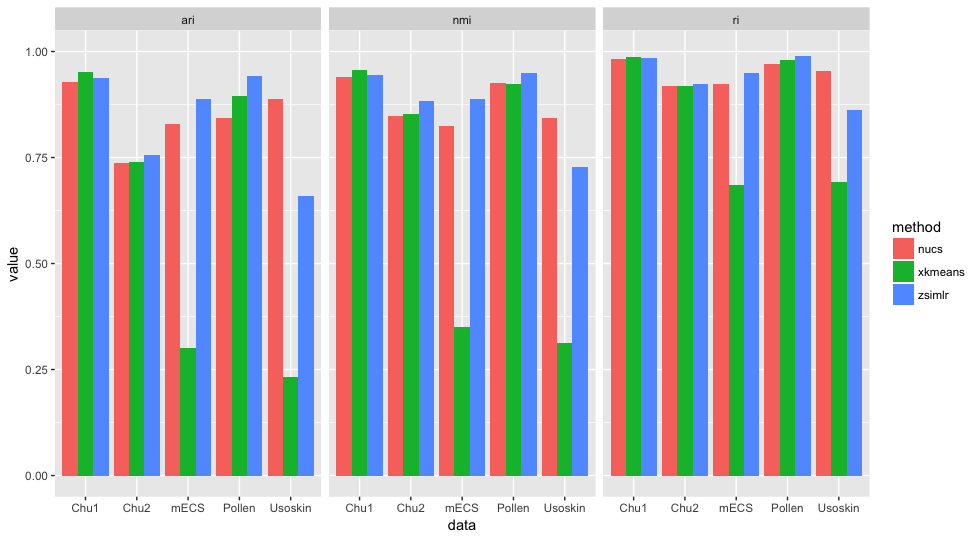
\includegraphics[width=0.98\linewidth]{initialization_no_nd.png}

We solve the following to get the underlying true similarity matrix $S$.
$$\min_{S,\sigma} \sum_{i=1}^{m} \frac{\|S-P_i\|_F^2}{2n^2 \sigma_i} + \tau \|S\|_1 + \sum_i \frac{\sigma_i}{2}$$
$S1 = 1, S\geq 0$.\\ 
We employ the scaled lasso to give different weights to each observed similarity $P_i$ and to control the noise level simultaneously. 

$$\mathcal{L} = \sum_{i=1}^{m} \frac{1}{2n^2 \sigma_i} \|Q-P_i\|_F^2 + \tau \|Q\|_1 + \sum_i \frac{\sigma_i}{2} + \langle Y, S-Q \rangle + \frac{\mu}{2} \|S-Q\|_F^2$$
\begin{itemize}
\item \textbf{update $Q$}\\
Defining $\phi = \mu + \sum_i \frac{1}{n^2 \sigma_i}$,
$$\mathcal{L}(Q) = \frac{\phi}{2} \norm{Q - \frac{1}{\phi} \left( \sum_i \frac{P_i}{n^2 \sigma_i} + Y + \mu S\right) }_F^2$$
Then soft-threshold the matrix element-wise.
\item \textbf{update $S$}
$$\mathcal{L}(S) = \norm{S-\left(Q-\frac{Y}{\mu}\right)}_F^2$$
where  $S\geq 0$ and $S1=1$
\item \textbf{update $\sigma$}
$$\sigma_i = \frac{\|P_i - Q\|_F^2}{n^2}$$
\end{itemize}
\noindent
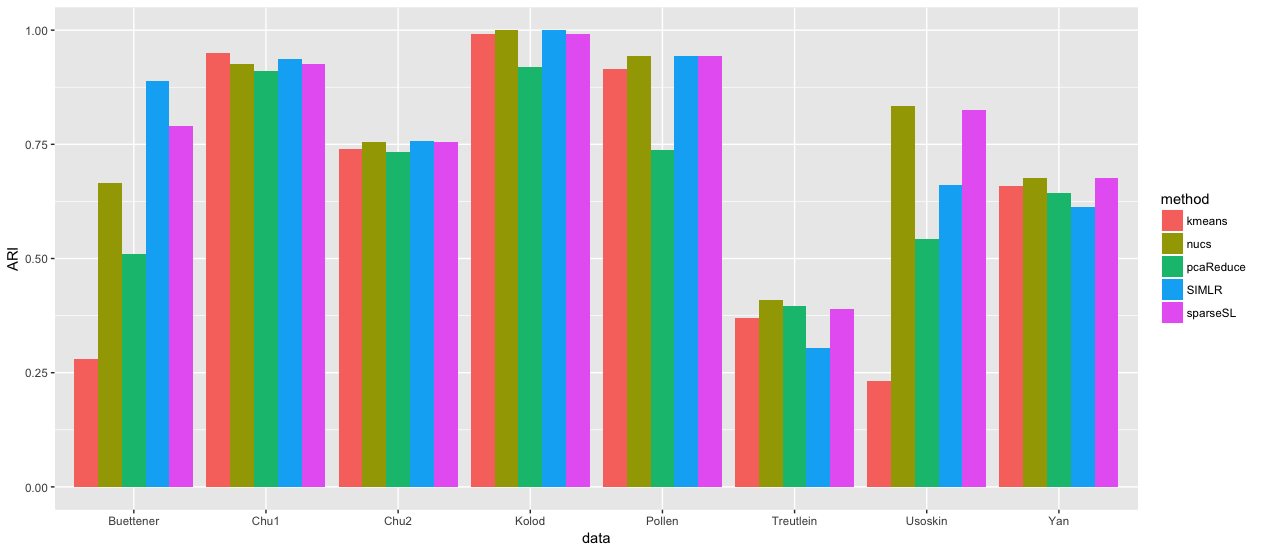
\includegraphics[width=0.98\linewidth]{results_2ndround.png}\\
\noindent
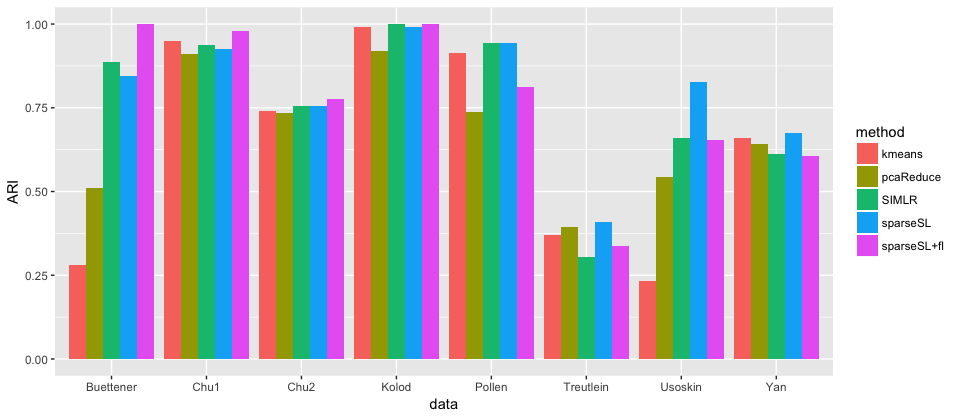
\includegraphics[width=0.98\linewidth]{fusedlassoresult.png}
\section*{Tuning parameter $\tau$}




\end{document}







